\documentclass[11pt]{article}

\usepackage[margin=1in]{geometry}
\usepackage[T1]{fontenc}
\usepackage{iftex}
\ifPDFTeX
  \usepackage[utf8]{inputenc}
\fi
\usepackage{amsmath,amssymb}
\usepackage{graphicx}
\usepackage{float}
\usepackage{booktabs}
\usepackage{array}
\usepackage{hyperref}
\usepackage{enumitem}

\hypersetup{colorlinks=true, linkcolor=black, urlcolor=blue, citecolor=black}
\setlist{nosep, leftmargin=1.5em}
\graphicspath{{figures/}}

% Allow clean float packing so pages do not suffer large blank gaps
\renewcommand{\topfraction}{0.90}
\renewcommand{\bottomfraction}{0.85}
\renewcommand{\textfraction}{0.08}
\renewcommand{\floatpagefraction}{0.80}
\setlength{\emergencystretch}{1.5em}

% --- Project Artifact URLs (Displayed on Page 1 per Section 2.2 Guidelines) ---
\newcommand{\RepoURL}{https://github.com/SufyanSiddiqui/ml-dkd-fall-2026}
\newcommand{\WeightsURL}{https://github.com/SufyanSiddiqui/ml-dkd-fall-2026/tree/main/outputs_final}
\newcommand{\LiveAppURL}{https://ml-dkd-fall-2026-36389and36374.streamlit.app}

\title{\textbf{Final Research Report}\\[0.35em]
\large Decoupled Knowledge Distillation on CIFAR-100:\\
From-Scratch Reproduction, Component \& Temperature Studies, and Live Deployment}
\author{Muhammad Sufyan Siddiqui (36389) \quad Muhammad Mudassir (36374)\\[0.3em]
\normalsize MS Data Science, Machine Learning (Fall 2026)}
\date{November 2026}

\begin{document}
\maketitle

\begin{center}
\small
\begin{tabular}{@{}lp{10.6cm}@{}}
\toprule
\textbf{Field} & \textbf{Details \& Public Artifact Links} \\
\midrule
Course \& Instructor & Machine Learning (Fall 2026), Dr.\ Rizwan Khan \\
Group Members & Muhammad Sufyan Siddiqui (36389), Muhammad Mudassir (36374) \\
Reference Paper & \emph{Decoupled Knowledge Distillation}, Borui Zhao, Quan Cui, Renjie Song, Yiyu Qiu, and Jiajun Liang, CVPR 2022, pp.\ 11953--11962 \cite{zhao2022} \\
Teacher $\rightarrow$ Student & CIFAR-100: \texttt{ResNet32$\times$4} ($7.43\text{M}$ params, $28.36\text{ MB}$) $\rightarrow$ \texttt{ResNet8$\times$4} ($1.23\text{M}$ params, $4.71\text{ MB}$) \\
Source Code Repository & \url{\RepoURL} \\
Trained Model Weights & \url{\WeightsURL} (11 full 240-epoch checkpoints + epoch logs) \\
Live Deployed Web App & \url{\LiveAppURL} (also runs offline locally via \texttt{streamlit run app.py}) \\
\bottomrule
\end{tabular}
\end{center}

\vspace{0.5em}
\noindent\textbf{Abstract.}
Classical knowledge distillation (KD) trains a compact student network to match the temperature-softened class probabilities of a larger teacher network through a single Kullback--Leibler (KL) divergence term. Zhao et al.\ (CVPR 2022) showed algebraically that this single KL term couples two distinct signals: binary target-class confidence (\(\mathrm{TCKD}\)) and the conditional distribution across the \(C-1\) non-target classes (\(\mathrm{NCKD}\)). Because classical KD multiplies \(\mathrm{NCKD}\) by \((1 - p_t^T)\), non-target dark knowledge is suppressed on the samples where the teacher is most confident. In this project, we implement the CIFAR-100 binary loader, residual architectures (\texttt{ResNet32$\times$4} and \texttt{ResNet8$\times$4}), classical KD, and Decoupled Knowledge Distillation (DKD) from scratch in PyTorch without importing the authors' library. Across eleven full 240-epoch GPU runs saved in \texttt{outputs\_final/}, our \texttt{ResNet8$\times$4} student improves from \(72.89\%\) (plain cross-entropy) and \(74.57\%\) (classical KD) to \(76.05\%\) and \(76.45\%\) across two independent DKD runs (\(76.25\%\) mean vs.\ \(76.32\%\) published). DKD closes roughly half of the recoverable teacher--student accuracy gap while compressing model size by \(6.03\times\) (\(28.36\text{ MB} \rightarrow 4.71\text{ MB}\)) with zero extra inference parameters. Three additional studies (component ablation, a temperature sweep over \(T \in \{1, 4, 10, 100\}\), and hardware step-time profiling) show that \(\mathrm{TCKD}\) alone drops accuracy below plain cross-entropy (\(68.73\%\)), \(\mathrm{NCKD}\) alone beats classical KD (\(75.31\%\)), and decoupling prevents classical KD's collapse at \(T=1\) (\(75.61\%\) vs.\ \(72.95\%\)). All eleven trained student checkpoints are deployed in an interactive Streamlit web application.

\tableofcontents
\clearpage

% =====================================================================
\section{Introduction and Problem Statement}
\label{sec:intro}

Deploying deep convolutional networks under tight memory and latency budgets creates a direct tradeoff between model size and accuracy. On 100-class CIFAR-100 image classification, a 32-layer wide residual network (\texttt{ResNet32$\times$4}, \(7{,}433{,}860\) parameters, \(28.36\text{ MB}\) in 32-bit floating point) reaches \(79.42\%\) top-1 test accuracy, whereas an 8-layer student from the same family (\texttt{ResNet8$\times$4}, \(1{,}233{,}540\) parameters, \(4.71\text{ MB}\)) reaches \(72.50\%\) when trained from hard labels alone \cite{zhao2022}. Recovering as much of that \(6.92\) percentage-point gap as possible without modifying the student at test time is the problem addressed by knowledge distillation \cite{bucilua2006,hinton2015}.

Following Hinton et al.\ \cite{hinton2015}, logit distillation supervises the student using only the teacher's output probability vector. For several years, logit distillation trailed intermediate feature-map methods such as FitNets \cite{romero2015}, Contrastive Representation Distillation (CRD) \cite{tian2020}, and ReviewKD \cite{chen2021}. Feature methods, however, require auxiliary projection layers, spatial connectors, or contrastive memory banks during training, tying the loss to internal layer dimensions.

Zhao et al.\ \cite{zhao2022} showed that output logits are not a weak supervision signal; rather, the classical KD loss couples target and non-target supervision in a harmful way. Because classical KD takes a single KL divergence across all \(C\) classes, the gradient carrying inter-class similarity among the \(C-1\) non-target classes is multiplied by \((1 - p_t^T)\), where \(p_t^T\) is the teacher's softened probability on the true class \(t\). On clear training examples where the teacher's ranking of visually related classes is most reliable, \(p_t^T\) approaches \(1\) and \((1 - p_t^T)\) approaches \(0\), switching off dark knowledge.

\textbf{Project Objectives.} This report documents four concrete deliverables:
\begin{enumerate}
    \item \textbf{From-Scratch Reproduction:} Implement the binary CIFAR-100 loader, \texttt{ResNet32$\times$4} and \texttt{ResNet8$\times$4} architectures, classical KD, and DKD in PyTorch, reproducing the published \(\texttt{ResNet32$\times$4} \to \texttt{ResNet8$\times$4}\) benchmark on the official test split.
    \item \textbf{Component Ablation Study:} Train isolated \(\mathrm{TCKD}\) (\(\alpha=1, \beta=0\)) and \(\mathrm{NCKD}\) (\(\alpha=0, \beta=8\)) students under identical initialization and optimization schedules to verify which term drives generalization.
    \item \textbf{Temperature Robustness \& Asymptotic Limit Study:} Compare classical KD and DKD across \(T \in \{1, 4, 10, 100\}\) and relate high-\(T\) behavior to the \(L_2\) logit-matching limit.
    \item \textbf{Model Deployment:} Serve the \(4.71\text{ MB}\) distilled student and reference teacher inside a public and locally runnable Streamlit inference application.
\end{enumerate}

% =====================================================================
\section{Literature Review and Background}
\label{sec:lit}

\subsection{Model Compression and Classical Knowledge Distillation}

A large convolutional network is usually more accurate than a small one, and it is also more expensive to store and to run. Bucilu\u{a}, Caruana, and Niculescu-Mizil framed that tradeoff in 2006 as model compression: train an expressive model, then train a smaller model to imitate it, so the small model can be deployed where the large one does not fit \cite{bucilua2006}. Deep residual networks made the gap concrete. He et al.\ showed that very deep residual nets set the accuracy standard on image classification, and they also made it obvious that the winning model is not the model one wants on a phone or under a tight latency budget \cite{he2016}.

Hinton, Vinyals, and Dean turned the compression idea into the training recipe later papers call knowledge distillation \cite{hinton2015}. A teacher network is trained in the usual way. A student, usually smaller, is trained with two signals at once: the hard class label, and the teacher's soft probability vector. The soft vector is the part they called \emph{dark knowledge}. A picture of a truck should not only be labeled ``truck.'' The teacher may also put a little mass on ``car'' and almost none on ``apple,'' and that ranking is useful. They control it with a temperature \(T\) inside the softmax. At \(T = 1\) the distribution is peaked. At \(T > 1\) the small probabilities on the wrong classes become visible, and the student is asked to match them with a KL divergence.

The extra cost is paid only at training time. At inference the teacher is discarded and the student runs alone. If the student is only a few points behind the teacher, most of the accuracy has been kept at a fraction of the compute.

\subsection{Logit Distillation and Feature Distillation}

After Hinton et al., the distillation literature split into two families \cite{zhao2022}:
\begin{itemize}
    \item \textbf{Logit distillation} stays on the teacher's \(C\)-dimensional output vector; the student never sees internal feature maps. Later logit papers mostly changed the training scheme around that same KL term rather than rewriting the objective. Deep Mutual Learning trains peer networks together so each acts as the other's teacher \cite{zhang2018}. Teacher-Assistant Knowledge Distillation (TAKD) inserts a mid-sized network when the teacher--student capacity gap is large \cite{mirzadeh2020}. Cho and Hariharan observed that more accurate, confident teachers often make worse classical-KD teachers and used early-stopped teachers as a workaround \cite{cho2019}, a failure mode later explained directly by the \((1 - p_t^T)\) factor in Equation~\eqref{eq:exact_kd}.
    \item \textbf{Feature distillation} matches intermediate representations instead of output logits. FitNets regress a student hidden map onto a teacher hint layer through a small learned adapter \cite{romero2015}. Attention Transfer (AT) aligns spatial attention summaries \cite{zagoruyko2017}. Relational Knowledge Distillation (RKD) compares distances and angles between sample pairs \cite{park2019}, and Contrastive Representation Distillation (CRD) pulls student and teacher embeddings of the same image together using a contrastive memory bank \cite{tian2020}. Overhaul of Feature Distillation (OFD) \cite{heo2019} and ReviewKD \cite{chen2021} refine cross-stage feature connectors. On CIFAR-100, CRD reaches \(75.51\%\) on \(\texttt{ResNet32$\times$4} \to \texttt{ResNet8$\times$4}\), but requires extra training parameters and intermediate feature taps.
\end{itemize}

Zhao et al.\ argued that logits sit at a higher semantic level than mid-network features and only underperformed because of the coupled classical loss. Decoupling the two terms pushed logit distillation to \(76.32\%\) on the same pair, beating CRD without auxiliary layers \cite{zhao2022}.

% =====================================================================
\section{Paper Methodology}
\label{sec:method}

\subsection{Algebraic Decomposition of Classical KD}

Consider \(C = 100\) classes. For an input image \(\mathbf{x}\) with true class \(t \in \{1, \dots, C\}\), let \(\mathbf{z}^T, \mathbf{z}^S \in \mathbb{R}^C\) denote the raw logits of the teacher and student. At temperature \(T > 0\), the softmax vector \(p = [p_1, \dots, p_C]\) for either network is:
\begin{equation}
p_i = \frac{\exp(z_i / T)}{\sum_{j=1}^{C} \exp(z_j / T)}, \qquad i \in \{1, \dots, C\}.
\end{equation}
Classical KD minimizes the temperature-scaled KL divergence between \(p^T\) and \(p^S\):
\begin{equation}
\mathcal{L}_{\mathrm{KD}} = T^2 \, \mathrm{KL}(p^T \parallel p^S) = T^2 \sum_{i=1}^{C} p_i^T \log \left(\frac{p_i^T}{p_i^S}\right),
\end{equation}
where \(T^2\) compensates for the \(1/T^2\) scaling of softmax logit gradients at high temperature.

Zhao et al.\ split the \(C\)-class distribution into two sub-distributions:
\begin{enumerate}
    \item \textbf{Binary Target vs.\ Non-Target Distribution} \(\mathbf{b} = [p_t, \, p_{\setminus t}] \in \mathbb{R}^2\), where \(p_{\setminus t} = \sum_{j \neq t} p_j = 1 - p_t\) is the combined probability on all \(C-1\) non-target classes.
    \item \textbf{Conditional Non-Target Distribution} \(\hat{\mathbf{p}} \in \mathbb{R}^{C-1}\), which renormalizes probability mass across only the 99 non-target classes (\(i \neq t\)):
    \begin{equation}
    \hat{p}_i = \frac{p_i}{p_{\setminus t}} = \frac{\exp(z_i / T)}{\sum_{j \neq t} \exp(z_j / T)}, \qquad \text{with } \sum_{i \neq t} \hat{p}_i = 1.
    \end{equation}
\end{enumerate}

Substituting \(p_i = p_{\setminus t} \, \hat{p}_i\) for every \(i \neq t\) inside the KL summation yields:
\begin{align}
\mathrm{KL}(p^T \parallel p^S)
&= p_t^T \log\left(\frac{p_t^T}{p_t^S}\right) + \sum_{i \neq t} p_{\setminus t}^T \hat{p}_i^T \log\left(\frac{p_{\setminus t}^T \hat{p}_i^T}{p_{\setminus t}^S \hat{p}_i^S}\right) \nonumber \\
&= p_t^T \log\left(\frac{p_t^T}{p_t^S}\right) + p_{\setminus t}^T \log\left(\frac{p_{\setminus t}^T}{p_{\setminus t}^S}\right)\underbrace{\sum_{i \neq t} \hat{p}_i^T}_{= 1} + p_{\setminus t}^T \sum_{i \neq t} \hat{p}_i^T \log\left(\frac{\hat{p}_i^T}{\hat{p}_i^S}\right) \nonumber \\
&= \underbrace{\mathrm{KL}(\mathbf{b}^T \parallel \mathbf{b}^S)}_{\mathrm{TCKD}} + (1 - p_t^T)\underbrace{\mathrm{KL}(\hat{\mathbf{p}}^T \parallel \hat{\mathbf{p}}^S)}_{\mathrm{NCKD}}.
\label{eq:exact_kd}
\end{align}

Equation~\eqref{eq:exact_kd} is an exact algebraic identity with zero approximations. In our code, we verified on 64-image CIFAR-100 batches that \(T^2(\mathrm{TCKD} + (1 - p_t^T)\mathrm{NCKD})\) matches standard \(\mathcal{L}_{\mathrm{KD}}\) to six decimal places (\(10.682806 = 10.682806\)).

\subsection{Why the Coupling Hurts and How DKD Fixes It}

Equation~\eqref{eq:exact_kd} identifies two structural problems in classical KD:
\begin{enumerate}
    \item \textbf{Suppression of Non-Target Dark Knowledge:} \(\mathrm{NCKD}\) captures visual similarity among the 99 non-target classes (e.g., ranking \texttt{lizard} and \texttt{dinosaur} far above \texttt{apple} on a \texttt{crocodile} image). Multiplying \(\mathrm{NCKD}\) by \((1 - p_t^T)\) shrinks this term toward zero whenever the teacher is confident (\(p_t^T \to 1\)).
    \item \textbf{Rigid Coupling Between Terms:} \(\mathrm{TCKD}\) conveys sample-level binary confidence, whereas \(\mathrm{NCKD}\) conveys relational class structure. Locking their weights to \((1, \, 1 - p_t^T)\) prevents tuning them independently; as shown in Section~\ref{sec:exp}, \(\mathrm{TCKD}\) on its own reduces test accuracy below plain cross-entropy.
\end{enumerate}

\textbf{Decoupled Knowledge Distillation (DKD)} replaces \((1, \, 1 - p_t^T)\) with independent constants \(\alpha \ge 0\) and \(\beta \ge 0\):
\begin{equation}
\mathcal{L}_{\mathrm{DKD}} = T^2 \big(\alpha \, \mathrm{TCKD} + \beta \, \mathrm{NCKD}\big),
\label{eq:dkd_final}
\end{equation}
giving the total student training loss with a 20-epoch linear warmup \(w(\text{epoch})\):
\begin{equation}
\mathcal{L}_{\mathrm{total}}(\text{epoch}) = \mathcal{L}_{\mathrm{CE}}(\mathbf{z}^S, t) + w(\text{epoch}) \, \mathcal{L}_{\mathrm{DKD}}(\mathbf{z}^S, \mathbf{z}^T, t), \qquad w(\text{epoch}) = \min\!\left(\frac{\text{epoch}}{20}, \, 1.0\right).
\label{eq:total_loss}
\end{equation}
Warming up \(w(\text{epoch})\) over the first 20 epochs prevents large \(\beta = 8.0\) distillation gradients from dominating random student weights at the start of training.

% =====================================================================
\section{Implementation Details}
\label{sec:impl}

\subsection{\texorpdfstring{Residual Network Architecture (\texttt{ResNet32$\times$4} and \texttt{ResNet8$\times$4})}{Residual Network Architecture (ResNet32x4 and ResNet8x4)}}

Both networks follow the 3-stage CIFAR ResNet design \cite{he2016} with a \(4\times\) channel width multiplier \([32, 64, 128, 256]\) (Figure~\ref{fig:arch_pipe}). Total learnable depth is \(6n + 2\): \(n = 5\) residual \texttt{BasicBlock}s per stage produces the 32-layer teacher (\texttt{ResNet32$\times$4}, \(7{,}433{,}860\) parameters), and \(n = 1\) block per stage produces the 8-layer student (\texttt{ResNet8$\times$4}, \(1{,}233{,}540\) parameters, a \(6.03\times\) reduction).

\begin{figure}[!htbp]
\centering
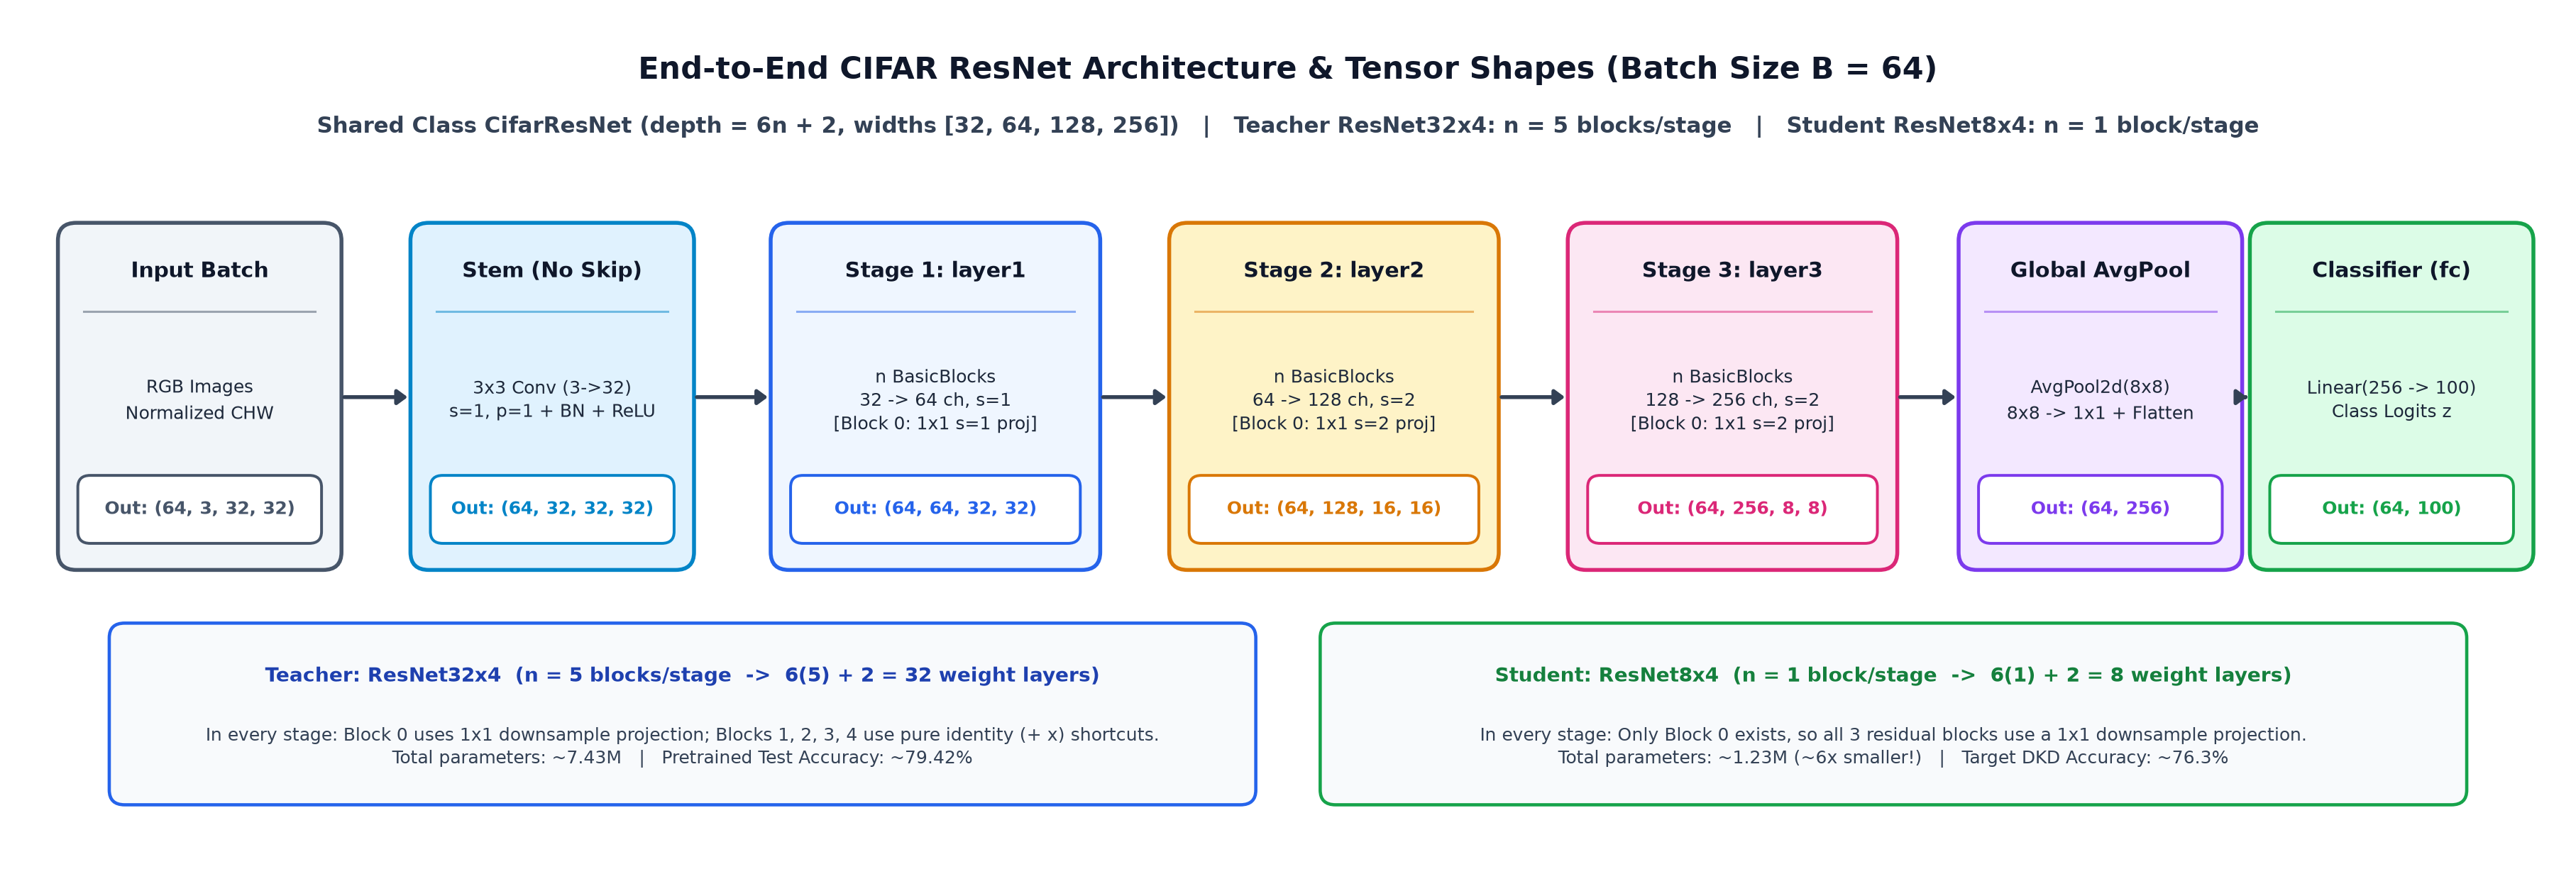
\includegraphics[width=0.94\textwidth]{cifar_resnet_pipeline.png}
\caption{End-to-end tensor pipeline for \texttt{CifarResNet} (\texttt{ResNet32$\times$4} teacher with \(n=5\) blocks/stage and \texttt{ResNet8$\times$4} student with \(n=1\) block/stage).}
\label{fig:arch_pipe}
\end{figure}

Every \texttt{nn.Conv2d} layer sets \texttt{bias=False} because \texttt{nn.BatchNorm2d} immediately follows each convolution, subtracting the per-channel batch mean and applying its own learnable shift. In our linear from-scratch notebook (\texttt{05\_dkd\_from\_scratch.ipynb}), convolutions use PyTorch's built-in Kaiming uniform initialization (\texttt{kaiming\_uniform\_}), whereas our modular package (\texttt{src/models/resnet.py}, used in \texttt{dkd\_T4\_seed2}) applies explicit fan-out Kaiming normal initialization matching \texttt{mdistiller}; because BatchNorm normalizes layer variance immediately, both initializations converge to the same accuracy band. As shown in Figure~\ref{fig:shortcuts} and Table~\ref{tab:stages}, Block 0 of each stage uses a \(1 \times 1\) projection shortcut (\texttt{downsample}) whenever channels double, while Blocks \(1 \dots 4\) in the teacher use parameter-free identity skip connections (\(+\mathbf{x}\)).

\begin{figure}[!htbp]
\centering
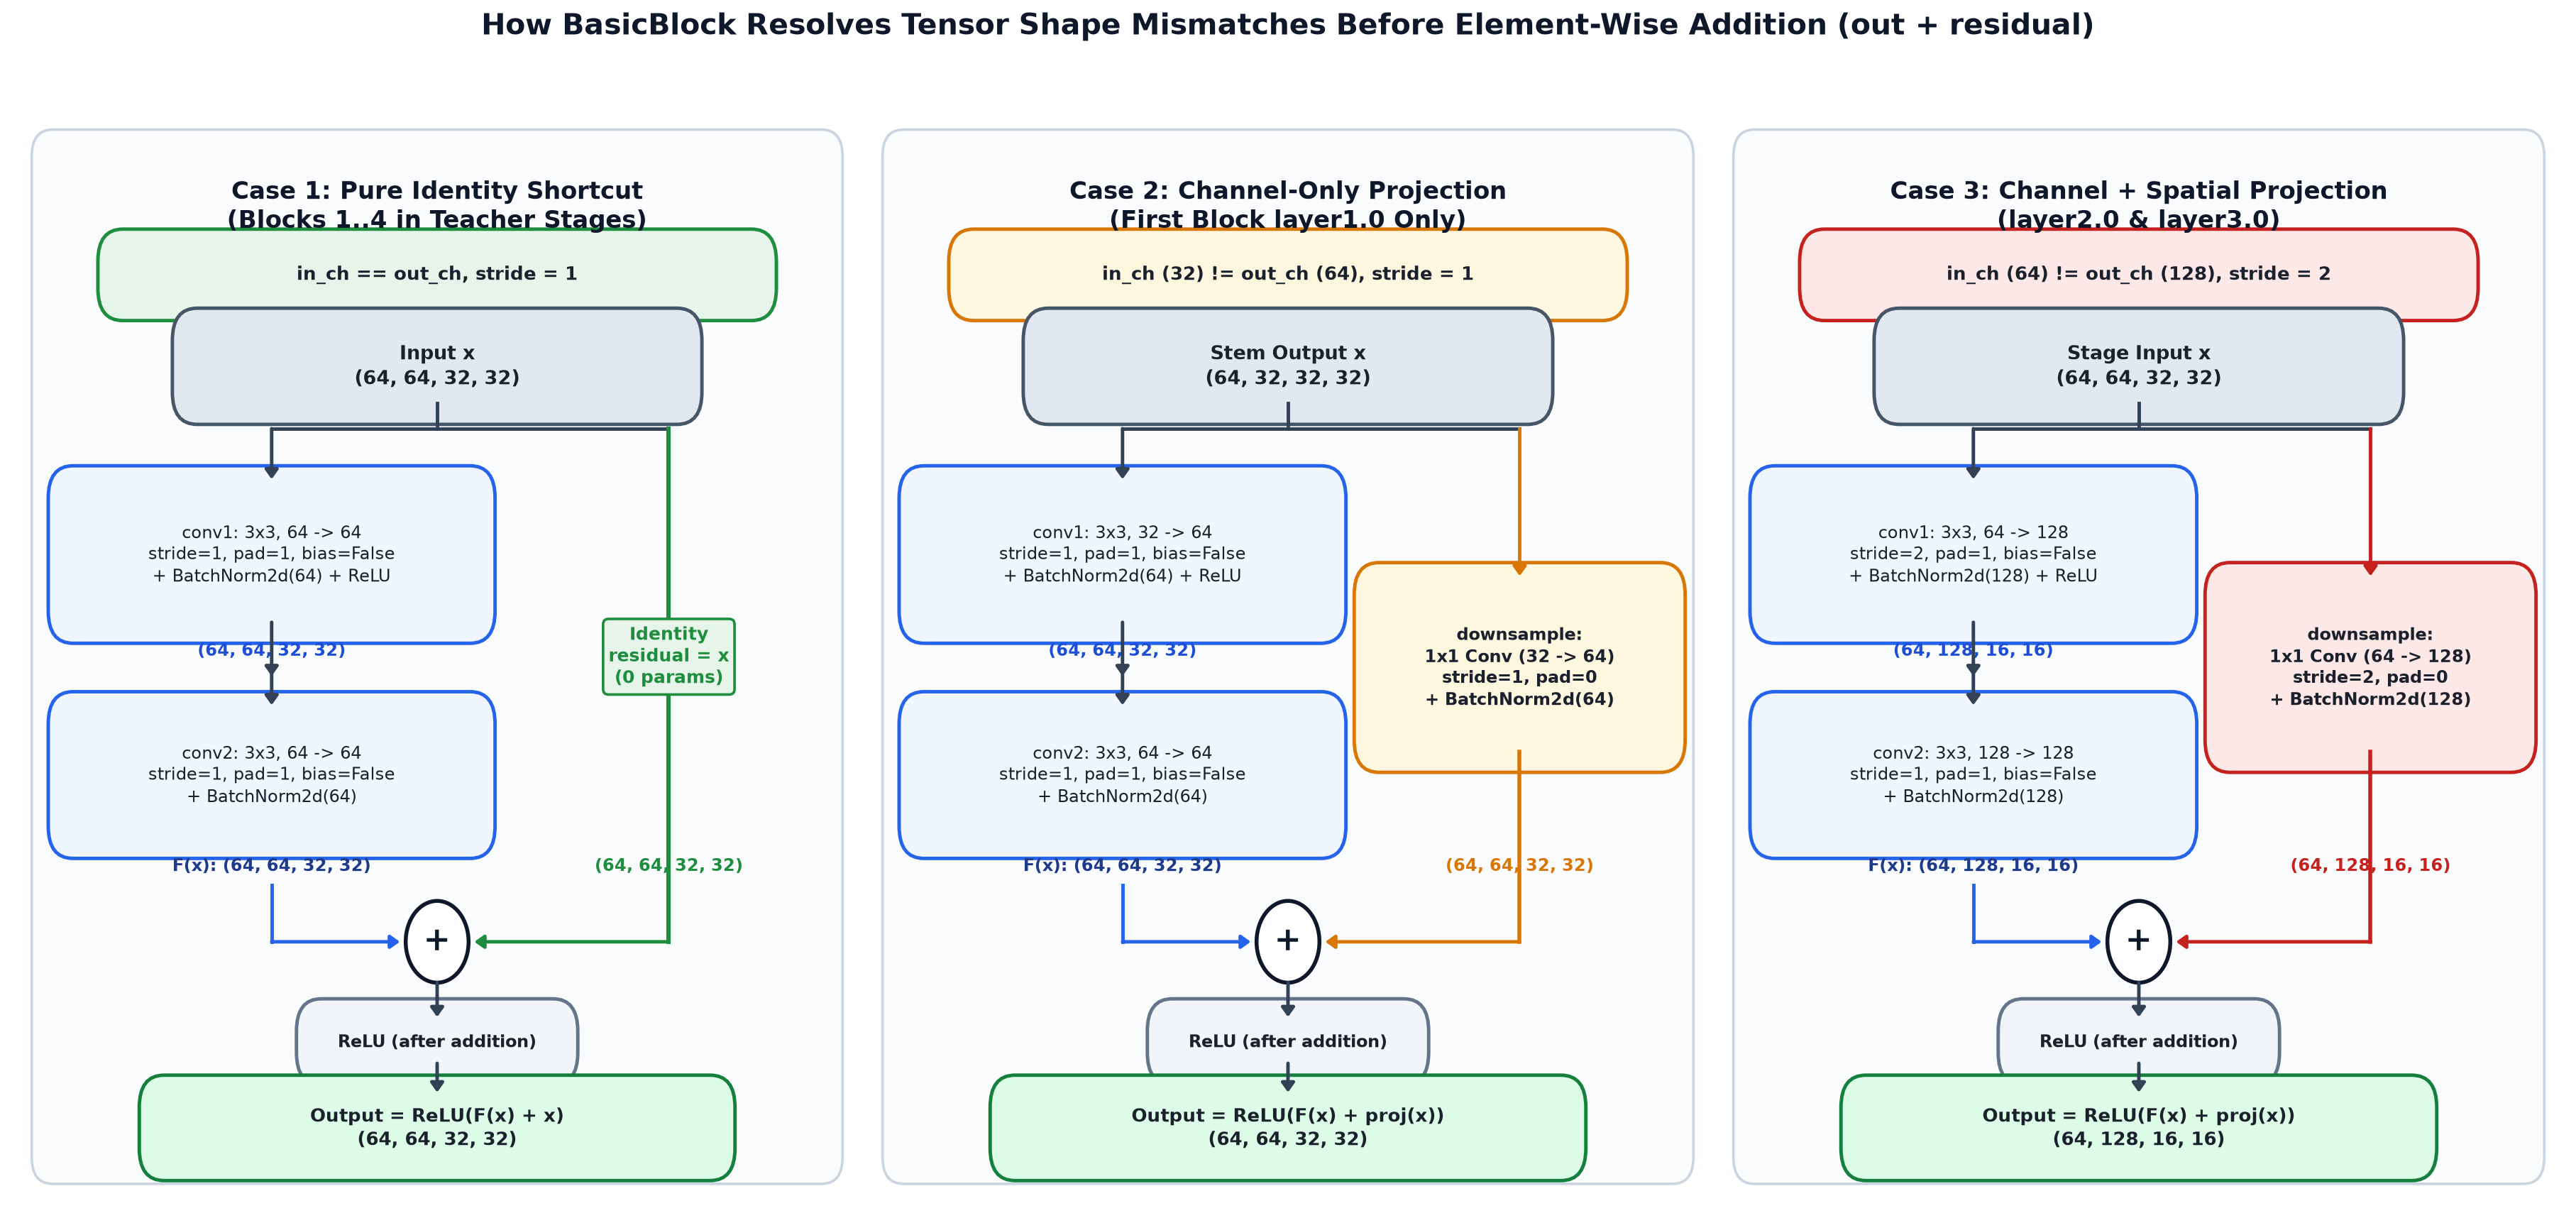
\includegraphics[width=0.90\textwidth]{resnet_shortcut_types.png}
\caption{Residual shortcut cases inside \texttt{BasicBlock}: identity skip, channel-only \(1\times 1\) projection (\texttt{layer1.0}), and strided spatial + channel \(1\times 1\) projection (\texttt{layer2.0}, \texttt{layer3.0}).}
\label{fig:shortcuts}
\end{figure}

\begin{table}[!htbp]
\centering
\small
\caption{Stage-by-stage batch tensor shapes (\(B = 64\)) for Teacher (\(n=5\)) and Student (\(n=1\)).}
\label{tab:stages}
\resizebox{\textwidth}{!}{%
\begin{tabular}{@{}llll@{}}
\toprule
\textbf{Stage} & \textbf{Input Tensor} & \textbf{Operations \& Shortcut Type} & \textbf{Output Tensor} \\
\midrule
Stem (\texttt{conv1+bn1}) & \((64, 3, 32, 32)\) & \(3\times 3\) conv (\(3\to 32, s=1, p=1\)) + BN + ReLU & \((64, 32, 32, 32)\) \\
\texttt{layer1} (\(n\) blocks) & \((64, 32, 32, 32)\) & Block 0: \(1\times 1\) proj (\(s=1\)); Blocks \(1..n{-}1\): Identity & \((64, 64, 32, 32)\) \\
\texttt{layer2} (\(n\) blocks) & \((64, 64, 32, 32)\) & Block 0: \(1\times 1\) proj (\(s=2\)); Blocks \(1..n{-}1\): Identity & \((64, 128, 16, 16)\) \\
\texttt{layer3} (\(n\) blocks) & \((64, 128, 16, 16)\) & Block 0: \(1\times 1\) proj (\(s=2\)); Blocks \(1..n{-}1\): Identity & \((64, 256, 8, 8)\) \\
Head (\texttt{avgpool+fc}) & \((64, 256, 8, 8)\) & \texttt{AvgPool2d(8)} $\rightarrow$ Flatten $\rightarrow$ \texttt{Linear(256, 100)} & \((64, 100)\) logits \\
\bottomrule
\end{tabular}}
\end{table}

\subsection{Numerical Stability in \texttt{NCKD} Logit Masking}

Computing \(\mathrm{NCKD} = \mathrm{KL}(\hat{\mathbf{p}}^T \parallel \hat{\mathbf{p}}^S)\) requires excluding the target class \(t\) without ragged tensor slicing or \(0 \cdot \log(0) = \mathrm{NaN}\) gradients. In both \texttt{05\_dkd\_from\_scratch.ipynb} and \texttt{src/losses/dkd.py}, we build a boolean mask via \texttt{scatter\_} and subtract \(1000.0\) from the scaled target logit before calling \texttt{F.softmax} and \texttt{F.log\_softmax}:
\[
\tilde{z}_i = \begin{cases} z_i / T - 1000.0, & i = t \\ z_i / T, & i \neq t \end{cases} \implies \exp(\tilde{z}_t) = e^{-1000} = 0.0 \text{ in IEEE-754 \texttt{float32}}.
\]
\texttt{F.softmax} then normalizes strictly over \(\sum_{j \neq t} \exp(z_j / T)\), while \texttt{F.kl\_div} evaluates \(0.0 \times (-1000) = 0.0\) without overflow or \(\mathrm{NaN}\) values even at \(T = 100.0\).

\subsection{Environment, Training Protocol, and Explicit Code Attribution}

\textbf{Environment \& Solver:} The primary 10-run suite (\texttt{SEED = 42}) was trained on Google Colab using an NVIDIA L4 GPU (24 GB VRAM, CUDA, two DataLoader workers, pinned memory, \(\approx 18.8\text{ ms/batch}\)), while \texttt{dkd\_T4\_seed2} ran on a Colab T4 GPU. Local verification and inference run on Apple Silicon (\texttt{mps}, Python 3.13, PyTorch 2.15.0, Streamlit 1.67.0, Plotly 7.1.0). Every run used SGD (\(\text{lr}=0.05\), \(\text{momentum}=0.9\), \(\text{weight\_decay}=5 \times 10^{-4}\)), batch size \(64\), \(240\) epochs, and step learning-rate drops (\(\times 0.1\)) at epochs \(150, 180,\) and \(210\).

\begin{table}[!htbp]
\centering
\small
\caption{Explicit Code, Weight, and Result Attribution (Deliverable 3 Section 2.4).}
\label{tab:attribution}
\begin{tabular}{@{}p{3.8cm}p{11.3cm}@{}}
\toprule
\textbf{Attribution Category} & \textbf{Exact Scope in This Project} \\
\midrule
\textbf{(a) Implemented by our team} & Binary CIFAR-100 byte parser, MD5 check, and NumPy/PyTorch transforms (\texttt{05\_dkd\_from\_scratch.ipynb}, \texttt{src/data/cifar100.py}); \texttt{BasicBlock}, \texttt{StudentResNet8x4}, and \texttt{TeacherResNet32x4}; \texttt{kd\_loss}, \texttt{tckd\_per\_sample}, \texttt{nckd\_per\_sample}, \texttt{dkd\_loss}, and 5-mode loss wrapper; 240-epoch training/resume loop; speed profiler; PNG exporter (\texttt{export\_test\_images.py}); and the Streamlit deployment app (\texttt{app.py}). Zero modules are imported from \texttt{mdistiller}. \\
\addlinespace[0.3em]
\textbf{(b) Adapted recipes \& conventions} & Solver hyperparameters (\(\text{lr}=0.05\), decay at \([150, 180, 210]\), batch size \(64\), weight decay \(5\times 10^{-4}\), 20-epoch warmup, \(\alpha=1.0, \beta=8.0, T=4.0\)), CIFAR channel constants, parameter naming, and the \(-1000\) logit-masking convention follow Zhao et al.\ and \texttt{mdistiller}'s \texttt{res32x4\_res8x4.yaml} so the teacher checkpoint loads with \texttt{strict=True} and results are comparable. \\
\addlinespace[0.3em]
\textbf{(c) Directly reused artifacts} & Only the pretrained frozen teacher checkpoint (\texttt{ckpt\_epoch\_240.pth}, \(79.42\%\) top-1) from \texttt{megvii-research/mdistiller} releases and Krizhevsky's official CIFAR-100 Python archive \cite{krizhevsky2009}. All 11 student checkpoints in \texttt{outputs\_final/} were trained from scratch by our team. \\
\addlinespace[0.3em]
\textbf{(d) Authors' vs.\ our results} & Every table and chart separates Zhao et al.'s published 5-trial averages \cite{zhao2022} from our reproduced test accuracies evaluated on the 10,000-image CIFAR-100 test split. \\
\bottomrule
\end{tabular}
\end{table}

\clearpage
% =====================================================================
\section{Dataset, Exploratory Data Analysis, and Preprocessing}
\label{sec:eda}

\subsection{Dataset Structure, Integrity, and Class Balance}

CIFAR-100 \cite{krizhevsky2009} is read from the official Python binary archive (\texttt{cifar-100-python.tar.gz}, MD5 \texttt{eb9058c3a382ffc7106e4002c42a8d85}). Extraction produces \texttt{train} (\(50{,}000\) images), \texttt{test} (\(10{,}000\) images), and \texttt{meta} (\(100\) fine classes grouped into \(20\) coarse superclasses of \(5\) fine classes each). Each image is stored as one row of \(3{,}072\) unsigned bytes (\(1{,}024\) red, \(1{,}024\) green, \(1{,}024\) blue), which our loader reshapes with \texttt{reshape(-1, 3, 32, 32)} followed by \texttt{transpose(0, 2, 3, 1)} to form \((32, 32, 3)\) RGB \texttt{uint8} arrays.

Table~\ref{tab:stats} and Figures~\ref{fig:balance}--\ref{fig:super} confirm exact class balance: every fine class has \(500\) training and \(100\) test images, and every superclass has \(2{,}500\) training images. Following the paper's CIFAR-100 protocol \cite{zhao2022}, we do not hold out a validation subset from the \(50{,}000\) training images; removing \(5{,}000\) images would train the student on \(45{,}000\) samples and break comparability with published benchmarks. Because every class has equal size, top-1 test accuracy is unbiased and serves as our evaluation metric.

\begin{table}[!htbp]
\centering
\small
\caption{Exact CIFAR-100 dataset statistics verified from extracted binary batches.}
\label{tab:stats}
\begin{tabular}{@{}lrlr@{}}
\toprule
\textbf{Quantity} & \textbf{Value} & \textbf{Quantity} & \textbf{Value} \\
\midrule
Training images & 50{,}000 & Validation split held out & 0 (official protocol) \\
Held-out test images & 10{,}000 & Image tensor dimensions & \(32 \times 32 \times 3\), \texttt{uint8} \([0, 255]\) \\
Fine classes (\(C\)) & 100 & Training / test per fine class & 500 / 100 \\
Coarse superclasses & 20 & Fine classes per superclass & 5 (2{,}500 train images) \\
\bottomrule
\end{tabular}
\end{table}

\begin{figure}[!htbp]
\centering
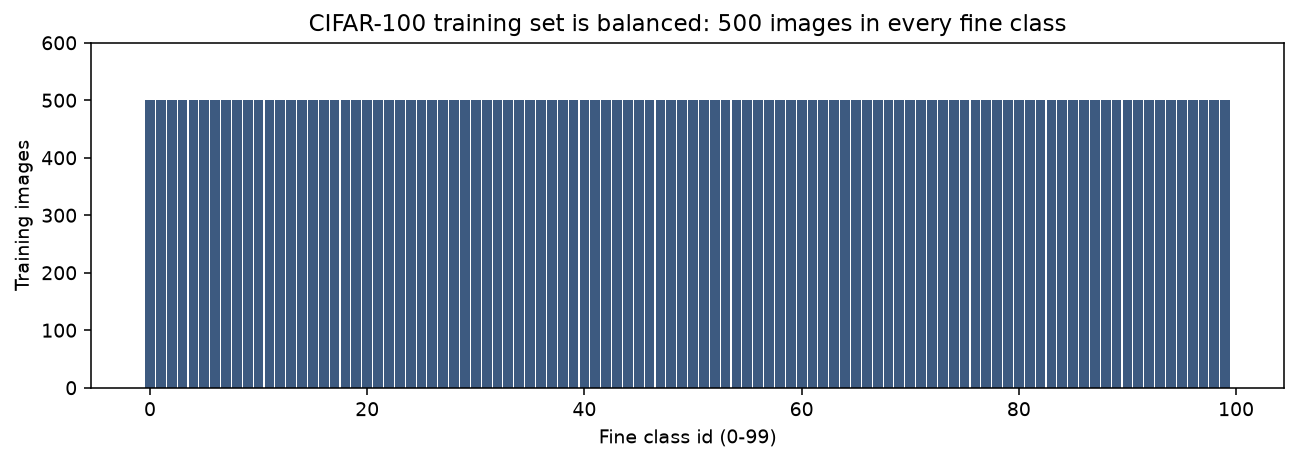
\includegraphics[width=0.86\textwidth]{class_balance.png}
\caption{Training sample count across all 100 fine classes (uniformly 500 images per class).}
\label{fig:balance}
\end{figure}

\begin{figure}[!htbp]
\centering
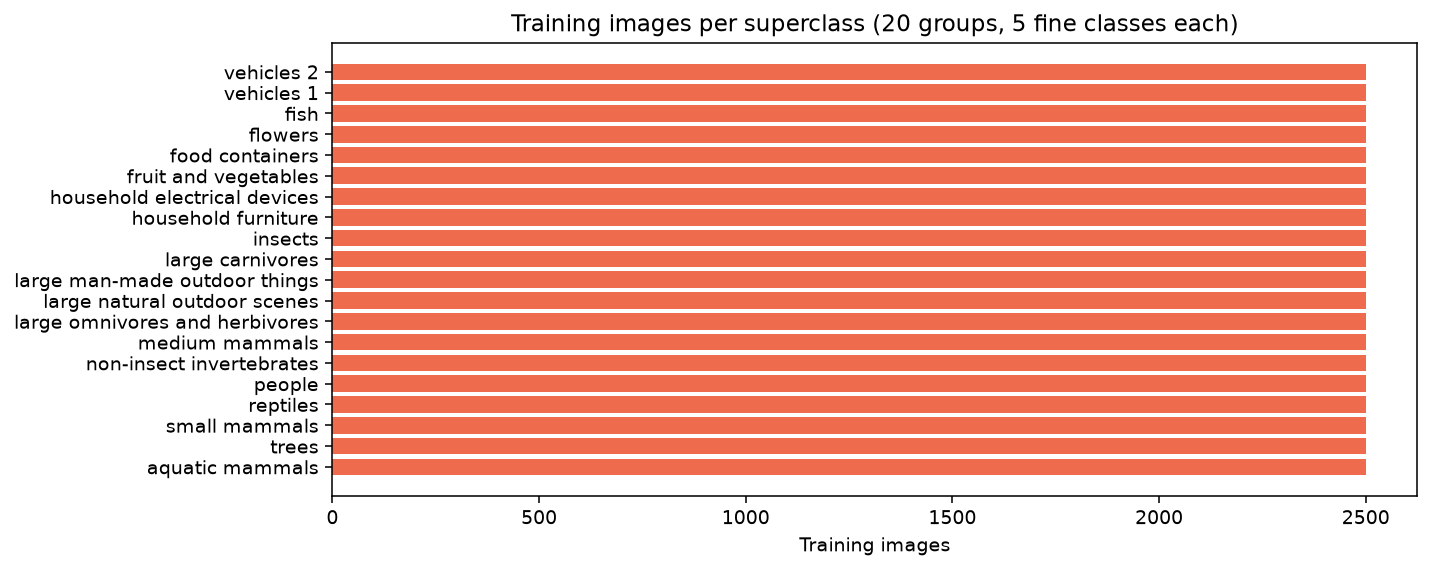
\includegraphics[width=0.74\textwidth]{superclass_counts.png}
\caption{Training sample count across all 20 coarse superclasses (uniformly 2{,}500 images per superclass).}
\label{fig:super}
\end{figure}

\subsection{Visual Inspection, Anomalies, Channel Moments, and Pixel-Space Overlap}

Figures~\ref{fig:raw} and \ref{fig:veh} show raw \(32 \times 32\) images across superclasses and inside \texttt{vehicles\_1} (\texttt{bicycle}, \texttt{bus}, \texttt{motorcycle}, \texttt{pickup\_truck}, \texttt{train}). Fine texture is largely absent at \(32 \times 32\), but shared coarse shape within a superclass explains why a trained teacher places non-zero probability on sibling classes, providing the signal captured by \(\mathrm{NCKD}\).

\begin{figure}[!htbp]
\centering
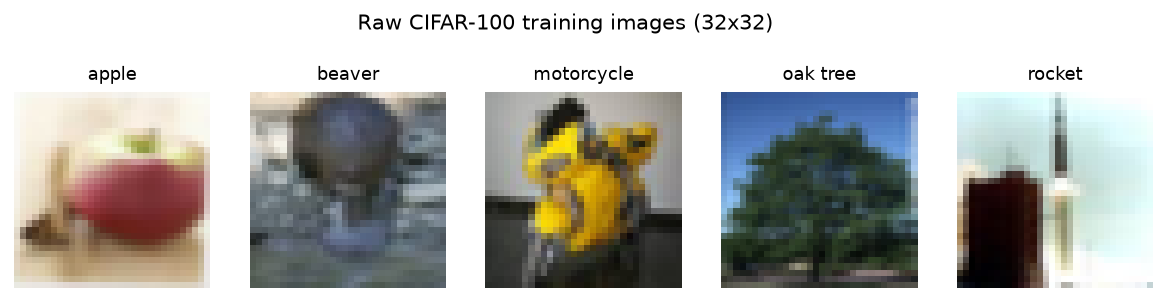
\includegraphics[width=0.86\textwidth]{raw_examples.png}
\caption{Raw \(32 \times 32\) training images from five distinct superclasses prior to augmentation or normalization.}
\label{fig:raw}
\end{figure}

\begin{figure}[!htbp]
\centering
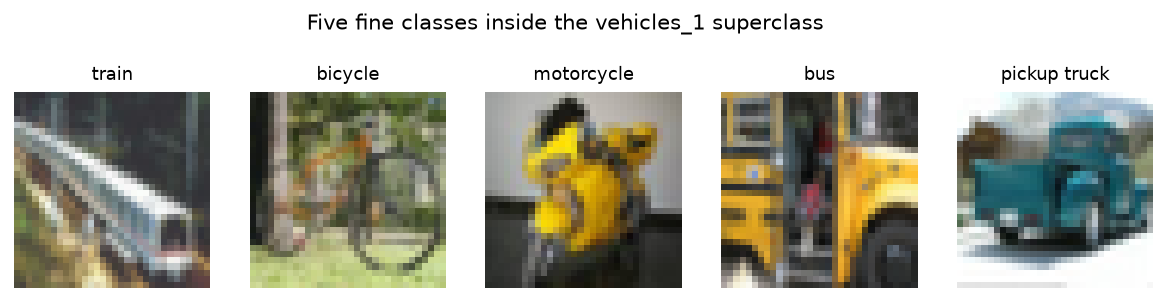
\includegraphics[width=0.86\textwidth]{superclass_vehicles.png}
\caption{Intra-superclass visual similarity across the five fine classes inside \texttt{vehicles\_1}.}
\label{fig:veh}
\end{figure}

Scans across all \(60{,}000\) rows found zero missing pixels, zero NaNs, and zero flat or single-channel images. Per-image brightness on \([0, 1]\) has a 1st percentile of \(0.168\), median \(0.464\), and 99th percentile \(0.872\) (Figure~\ref{fig:bright}). Byte-level checks found 14 repeated training rows, 2 repeated test rows, and 10 cross-split copies; all rows are kept so the evaluation split matches the official benchmark.

Recomputing RGB moments on the \(50{,}000\) training images gives \(\mu = (0.5071, 0.4865, 0.4409)\) and \(\sigma = (0.2673, 0.2564, 0.2762)\), matching the recipe constants \((0.5071, 0.4867, 0.4408)\) and \((0.2675, 0.2565, 0.2761)\) to three decimals (Figure~\ref{fig:hist}). Principal Component Analysis (PCA) on \(4{,}000\) raw pixel vectors keeps \(41.9\%\) variance in the first two axes (\(85\) axes for \(90\%\)) and shows heavy class overlap across both superclasses and \texttt{vehicles\_1} (Figures~\ref{fig:pca}--\ref{fig:pcav}), confirming that linear pixel classifiers are inadequate.

\begin{figure}[!htbp]
\centering
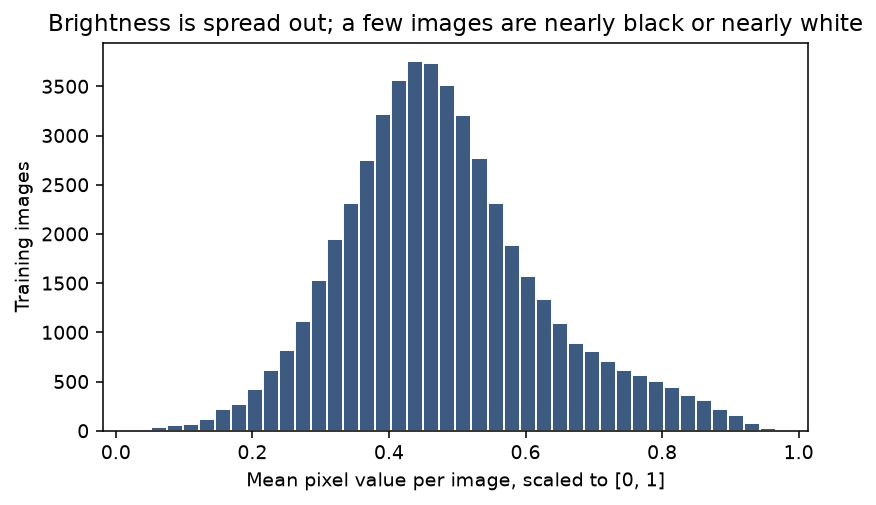
\includegraphics[width=0.66\textwidth]{brightness.png}
\caption{Distribution of mean per-image brightness across the 50{,}000 training images.}
\label{fig:bright}
\end{figure}

\begin{figure}[!htbp]
\centering
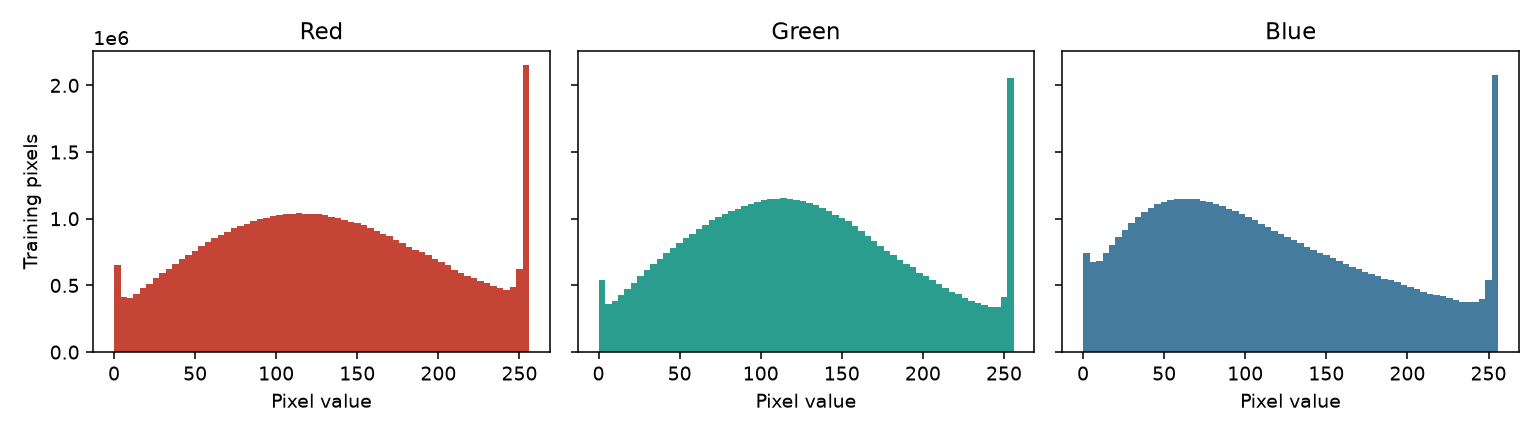
\includegraphics[width=0.92\textwidth]{channel_histograms.png}
\caption{Per-channel RGB pixel intensity histograms across the CIFAR-100 training split.}
\label{fig:hist}
\end{figure}

\begin{figure}[!htbp]
\centering
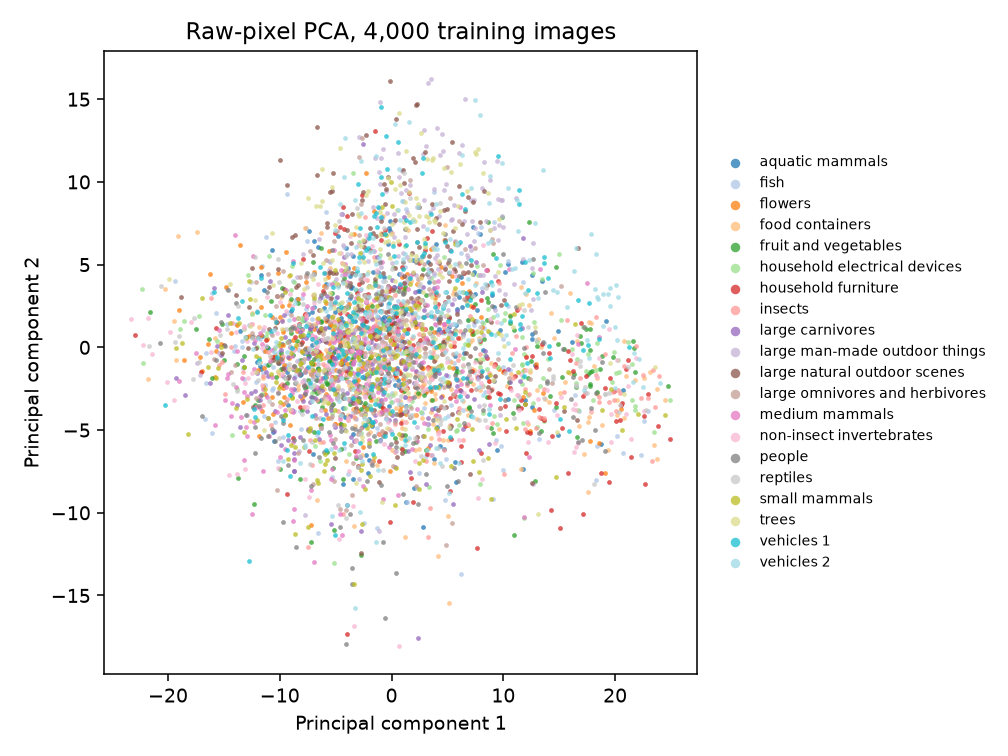
\includegraphics[width=0.82\textwidth]{pca_superclasses.png}
\caption{Projection of 4{,}000 raw training images onto the first two principal components, colored by superclass.}
\label{fig:pca}
\end{figure}

\begin{figure}[!htbp]
\centering
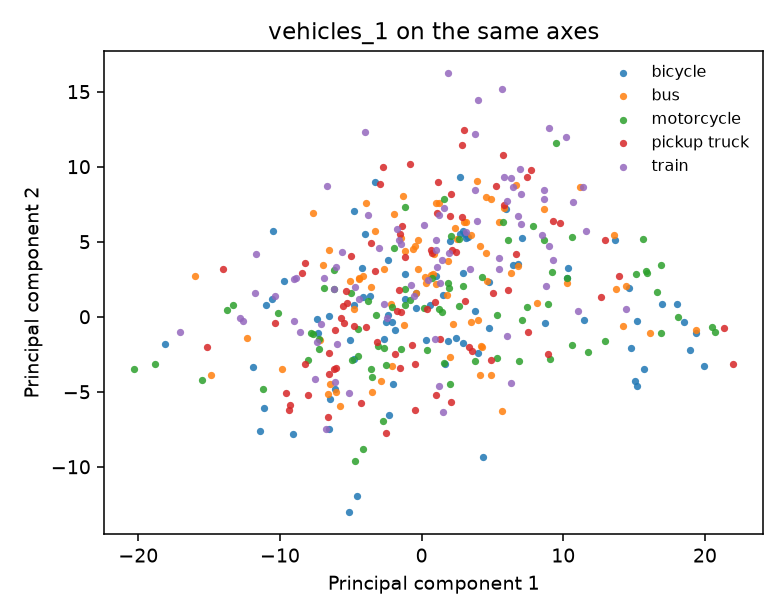
\includegraphics[width=0.66\textwidth]{pca_vehicles.png}
\caption{Overlap of the five \texttt{vehicles\_1} fine classes in raw 2D PCA pixel space.}
\label{fig:pcav}
\end{figure}

\subsection{Training and Evaluation Preprocessing Pipeline}

\begin{itemize}
    \item \textbf{Training transform (\texttt{preprocess\_train}):} Pad each \(32 \times 32\) image by \(4\) zero pixels on each border (\(40 \times 40\)), take a random \(32 \times 32\) crop, flip horizontally with probability \(0.5\), divide by \(255\), normalize per channel by \(\mu, \sigma\), and transpose to contiguous \texttt{float32} CHW \((3, 32, 32)\) (Figure~\ref{fig:prep}).
    \item \textbf{Evaluation \& live deployment transform (\texttt{preprocess\_eval}):} Resize non-\(32\times 32\) user uploads bilinearly to \(32 \times 32\) RGB, divide by \(255\), normalize with the same \(\mu, \sigma\), and output CHW \((1, 3, 32, 32)\) with no random crop or flip.
\end{itemize}

\begin{figure}[!htbp]
\centering
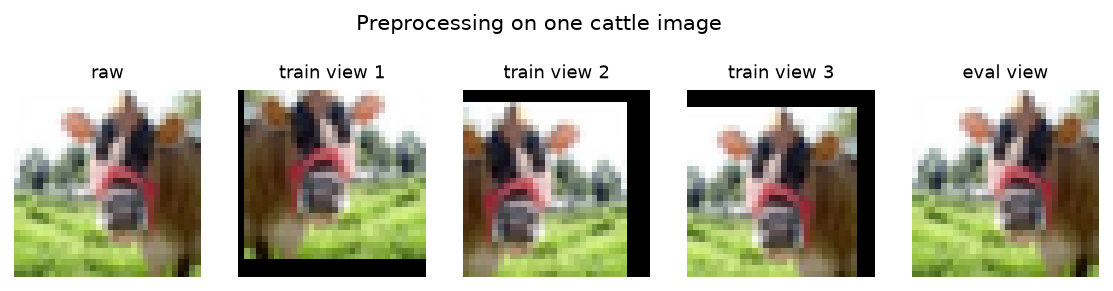
\includegraphics[width=0.92\textwidth]{preprocess_views.png}
\caption{One CIFAR-100 image shown raw, across three stochastic training augmentations, and under deterministic evaluation preprocessing.}
\label{fig:prep}
\end{figure}

\clearpage
% =====================================================================
\section{Reproduction Results}
\label{sec:repro}

Table~\ref{tab:repro} compares our from-scratch PyTorch runs against Zhao et al.'s published CIFAR-100 benchmarks for \(\texttt{ResNet32$\times$4} \to \texttt{ResNet8$\times$4}\) \cite{zhao2022}. The original paper reports classical KD in two places: \(73.33\%\) in Table~6 under standard \(0.1\,\mathcal{L}_{\mathrm{CE}} + 0.9\,\mathcal{L}_{\mathrm{KD}}\) weights, and \(73.63\%\) in Table~1 under unit weights \(1.0\,\mathcal{L}_{\mathrm{CE}} + 1.0\,\mathcal{L}_{\mathrm{KD}}\). To keep the \(\mathcal{L}_{\mathrm{CE}}\) weight (\(1.0\)) identical between classical KD and DKD without introducing a \(10\times\) cross-entropy weight change as a confounding variable, \texttt{kd\_T4} uses the exact unit-weight setup of Paper Table~1. Both independent DKD runs (\texttt{dkd\_T4} and \texttt{dkd\_T4\_seed2}) are archived in \texttt{outputs\_final/}.

\begin{table}[!htbp]
\centering
\small
\caption{CIFAR-100 Method Reproduction: Published Benchmarks vs.\ Audited Checkpoints in \texttt{outputs\_final/}.}
\label{tab:repro}
\resizebox{\textwidth}{!}{%
\begin{tabular}{@{}llcccc@{}}
\toprule
\textbf{Model / Method} & \textbf{Run ID (\texttt{outputs\_final/})} & \textbf{Paper Top-1} & \textbf{Our Best Top-1} & \textbf{Last-20 Ep Mean} & \textbf{Teacher Gap Closed} \\
\midrule
Teacher (\texttt{ResNet32$\times$4}, frozen) & \texttt{teacher} & \(79.42\%\) & \textbf{79.42\%} & \(79.42\%\) & \(100.0\%\) (Ceiling) \\
Student Baseline (Plain CE) & \texttt{ce} & \(72.50\%\) & \textbf{72.89\%} & \(72.51\%\) & \(0.0\%\) (Baseline) \\
Classical KD (\(T=4.0\), unit wt.) & \texttt{kd\_T4} & \(73.63\%\)$^\dagger$ & \textbf{74.57\%} & \(74.30\%\) & \(+25.7\%\) \\
\textbf{Decoupled KD (\(\alpha=1, \beta=8, T=4\))} & \texttt{dkd\_T4} (Seed 1) & \(76.32\%\) & \textbf{76.05\%} & \(75.87\%\) & \textbf{+48.4\%} \\
\textbf{Decoupled KD (\(\alpha=1, \beta=8, T=4\))} & \texttt{dkd\_T4\_seed2} (Seed 2) & \(76.32\%\) & \textbf{76.45\%} & \(76.19\%\) & \textbf{+54.5\%} \\
\midrule
\emph{Two-Seed DKD Mean (\(T=4.0\))} & \emph{Mean of Seeds 1 \& 2} & \emph{76.32\%} & \textbf{76.25\%} & \emph{76.03\%} & \textbf{+51.5\%} \\
\bottomrule
\multicolumn{6}{@{}l}{\footnotesize $^\dagger$Paper Table~1 reports \(73.63\%\) for \(1.0\,\text{CE}+1.0\,\text{KD}\); Paper Table~6 reports \(73.33\%\) for \(0.1\,\text{CE}+0.9\,\text{KD}\).}
\end{tabular}}
\end{table}

As shown in Figures~\ref{fig:repro_curves} and \ref{fig:dkd_loss}, the published ranking holds across every baseline:
\[
\text{Plain CE }(72.89\%) < \text{Classical KD }(74.57\%) < \text{DKD }(76.05\% \text{ \& } 76.45\%) < \text{Teacher }(79.42\%).
\]
The converged last-20-epoch average of \texttt{ce} is \(72.51\%\) (vs.\ \(72.50\%\) published), and our two \(T=4.0\) DKD checkpoints average \(76.25\%\) (\(-0.07\%\) from the paper's 5-trial mean of \(76.32\%\)). During Epochs 1--149 at \(\text{lr}=0.05\), test accuracy stays near \(58\%\text{--}63\%\); at Epoch 150, dropping the learning rate to \(0.005\) produces an immediate \(+12\%\text{--}14\%\) jump across all runs.

\begin{figure}[!htbp]
\centering
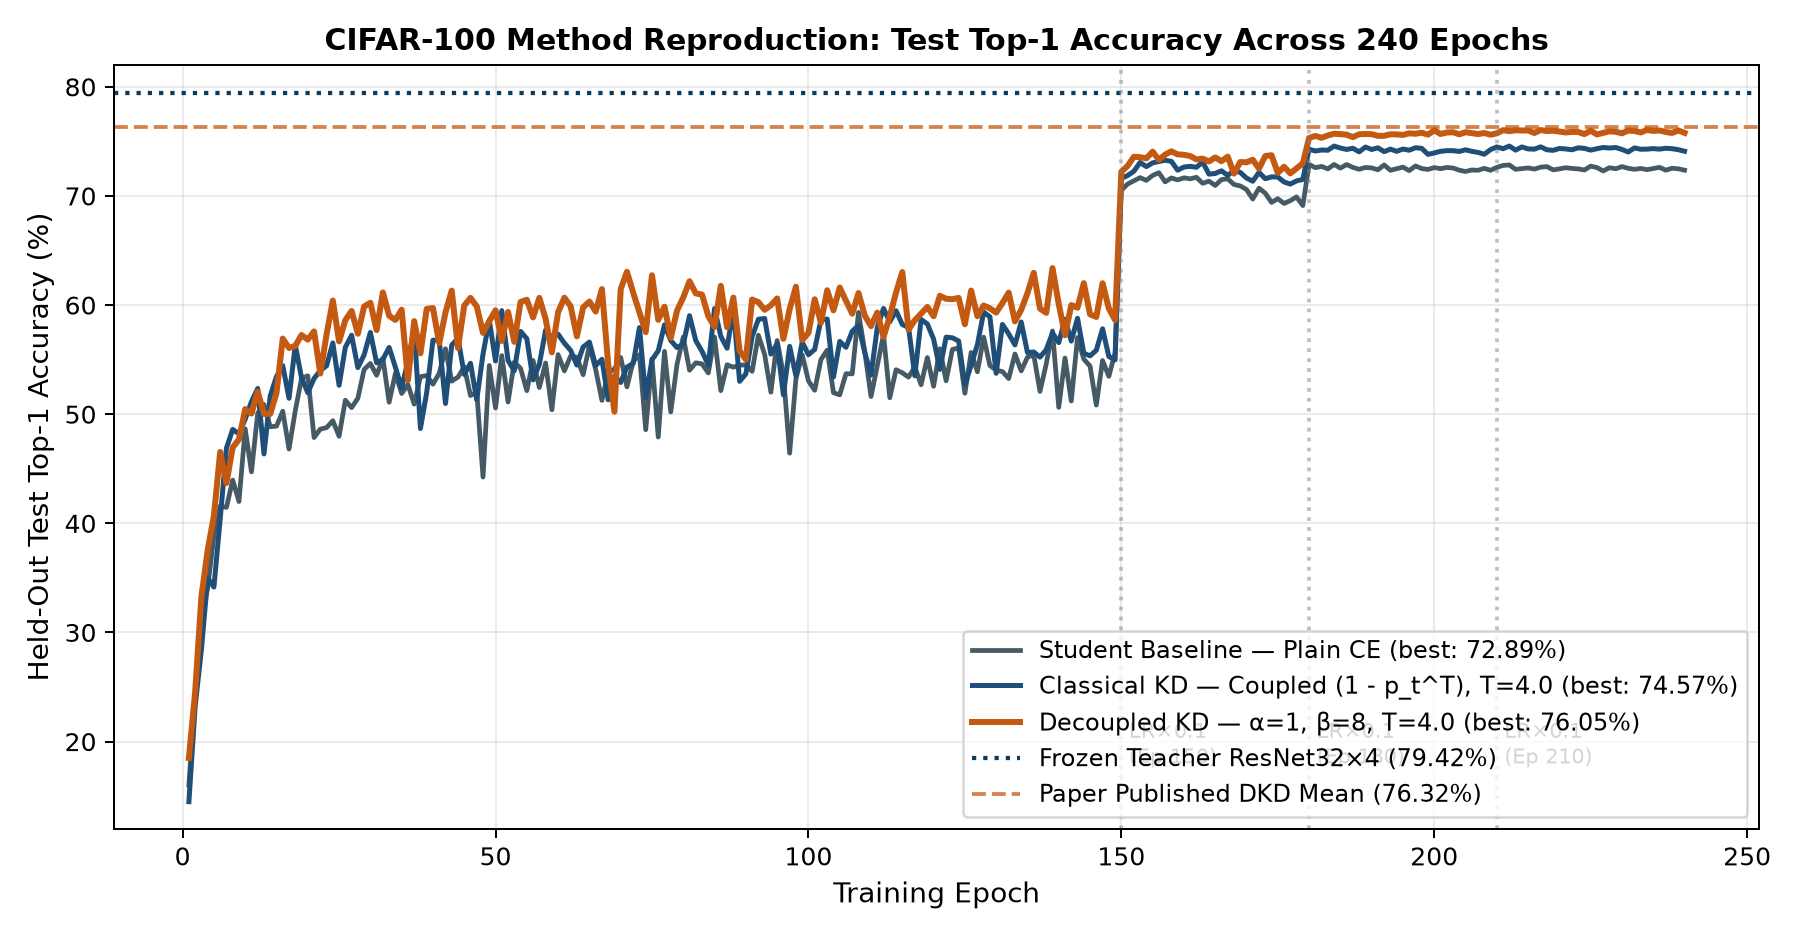
\includegraphics[width=0.92\textwidth]{reproduction_curves.png}
\caption{240-epoch CIFAR-100 test top-1 accuracy curves for Plain CE, Classical KD (\(T=4\)), and Decoupled KD (\texttt{dkd\_T4}, \(T=4\)) against the frozen \texttt{ResNet32$\times$4} teacher.}
\label{fig:repro_curves}
\end{figure}

\begin{figure}[!htbp]
\centering
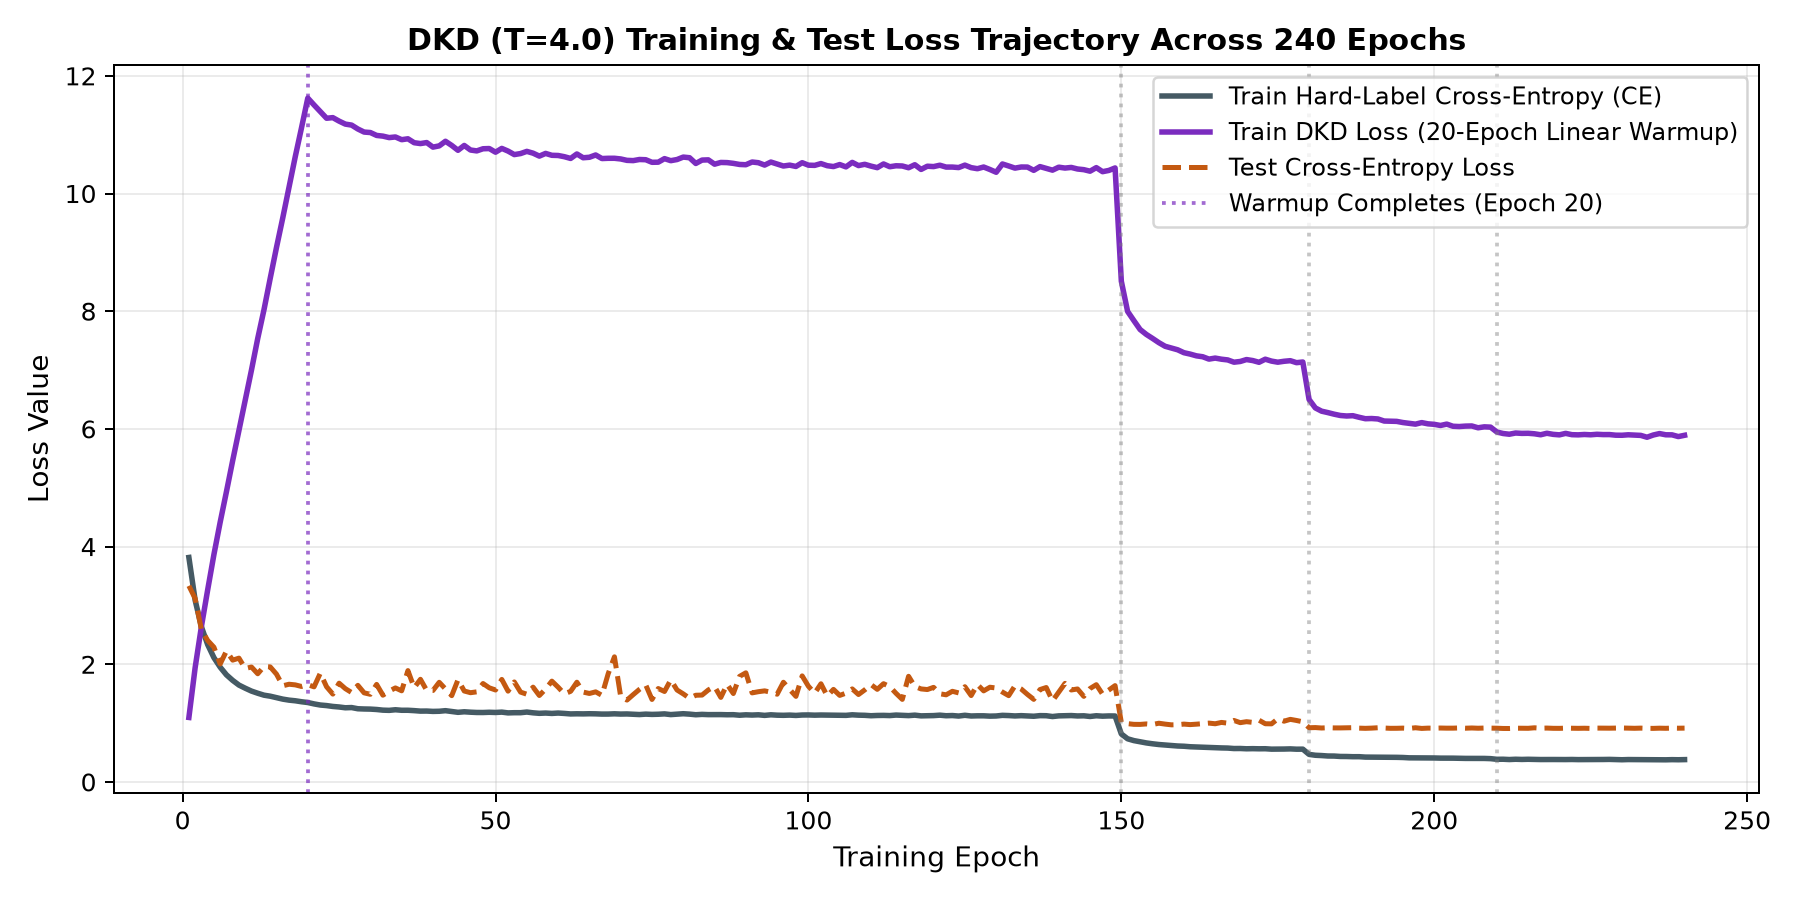
\includegraphics[width=0.90\textwidth]{dkd_loss_decomposition.png}
\caption{Loss trajectory during \texttt{dkd\_T4} training, showing the 20-epoch linear distillation warmup and convergence steps at Epochs 150, 180, and 210.}
\label{fig:dkd_loss}
\end{figure}

\clearpage
% =====================================================================
\section{Additional Experiments}
\label{sec:exp}

Beyond reproduction, we ran three additional experiments (seven further 240-epoch GPU runs plus step-time profiling) to test DKD's component behavior, temperature sensitivity, and compute cost.

\subsection{\texorpdfstring{Study 1: Decoupled Component Ablation (\texttt{TCKD} Only vs.\ \texttt{NCKD} Only)}{Study 1: Decoupled Component Ablation (TCKD Only vs. NCKD Only)}}

\begin{itemize}
    \item \textbf{Research Question:} Which decoupled component drives student generalization, and how does each term behave when the other is switched off?
    \item \textbf{Setup:} Keeping \texttt{SEED=42}, SGD schedule, \(T=4.0\), \(1.0\,\mathcal{L}_{\mathrm{CE}}\), and the 20-epoch warmup unchanged from \texttt{dkd\_T4}, we trained \texttt{tckd\_only\_T4} (\(\alpha=1.0, \beta=0.0\)) and \texttt{nckd\_only\_T4} (\(\alpha=0.0, \beta=8.0\)).
    \item \textbf{Results (Table~\ref{tab:ablation}, Figures~\ref{fig:ablation_curves}--\ref{fig:bars_all}):} Removing non-target dark knowledge (\texttt{tckd\_only\_T4}) drops accuracy to \(68.73\%\), which is \(4.16\) percentage points \emph{worse} than training with no teacher (\texttt{ce}: \(72.89\%\)) and within \(0.10\%\) of the paper's \(68.63\%\). Conversely, keeping only non-target dark knowledge (\texttt{nckd\_only\_T4}) reaches \(75.31\%\), matching Paper Table~3 (\(75.30\%\)) to one test image out of \(10{,}000\) and beating Classical KD (\(74.57\%\)) by \(+0.74\%\). Combining both terms (\(\alpha=1, \beta=8\)) adds another \(+0.74\%\) to reach \(76.05\%\).
\end{itemize}

\begin{table}[!htbp]
\centering
\small
\caption{Study 1: Component Ablation Results on CIFAR-100 (\texttt{SEED=42}, \(T = 4.0\), 240 Epochs).}
\label{tab:ablation}
\resizebox{\textwidth}{!}{%
\begin{tabular}{@{}lcccccc@{}}
\toprule
\textbf{Configuration} & \textbf{\(\alpha\)} & \textbf{\(\beta\)} & \textbf{Paper Top-1} & \textbf{Our Best Top-1} & \textbf{\(\Delta\) vs.\ CE} & \textbf{Ep 240 Train Acc} \\
\midrule
Plain CE (No Teacher) & \(0\) & \(0\) & \(72.50\%\) & \(72.89\%\) & \(0.00\%\) & \(95.32\%\) \\
\texttt{tckd\_only\_T4} (Target Only) & \(1.0\) & \(0.0\) & \(68.63\%\) & \textbf{68.73\%} & \(-4.16\%\) & \(91.58\%\) \\
\texttt{nckd\_only\_T4} (Dark Knowledge Only) & \(0.0\) & \(8.0\) & \(75.30\%\) & \textbf{75.31\%} & \(+2.42\%\) & \(88.32\%\) \\
Full \texttt{dkd\_T4} (Balanced) & \(1.0\) & \(8.0\) & \(76.32\%\) & \textbf{76.05\%} & \(+3.16\%\) & \(90.02\%\) \\
\bottomrule
\end{tabular}}
\end{table}

\begin{figure}[!htbp]
\centering
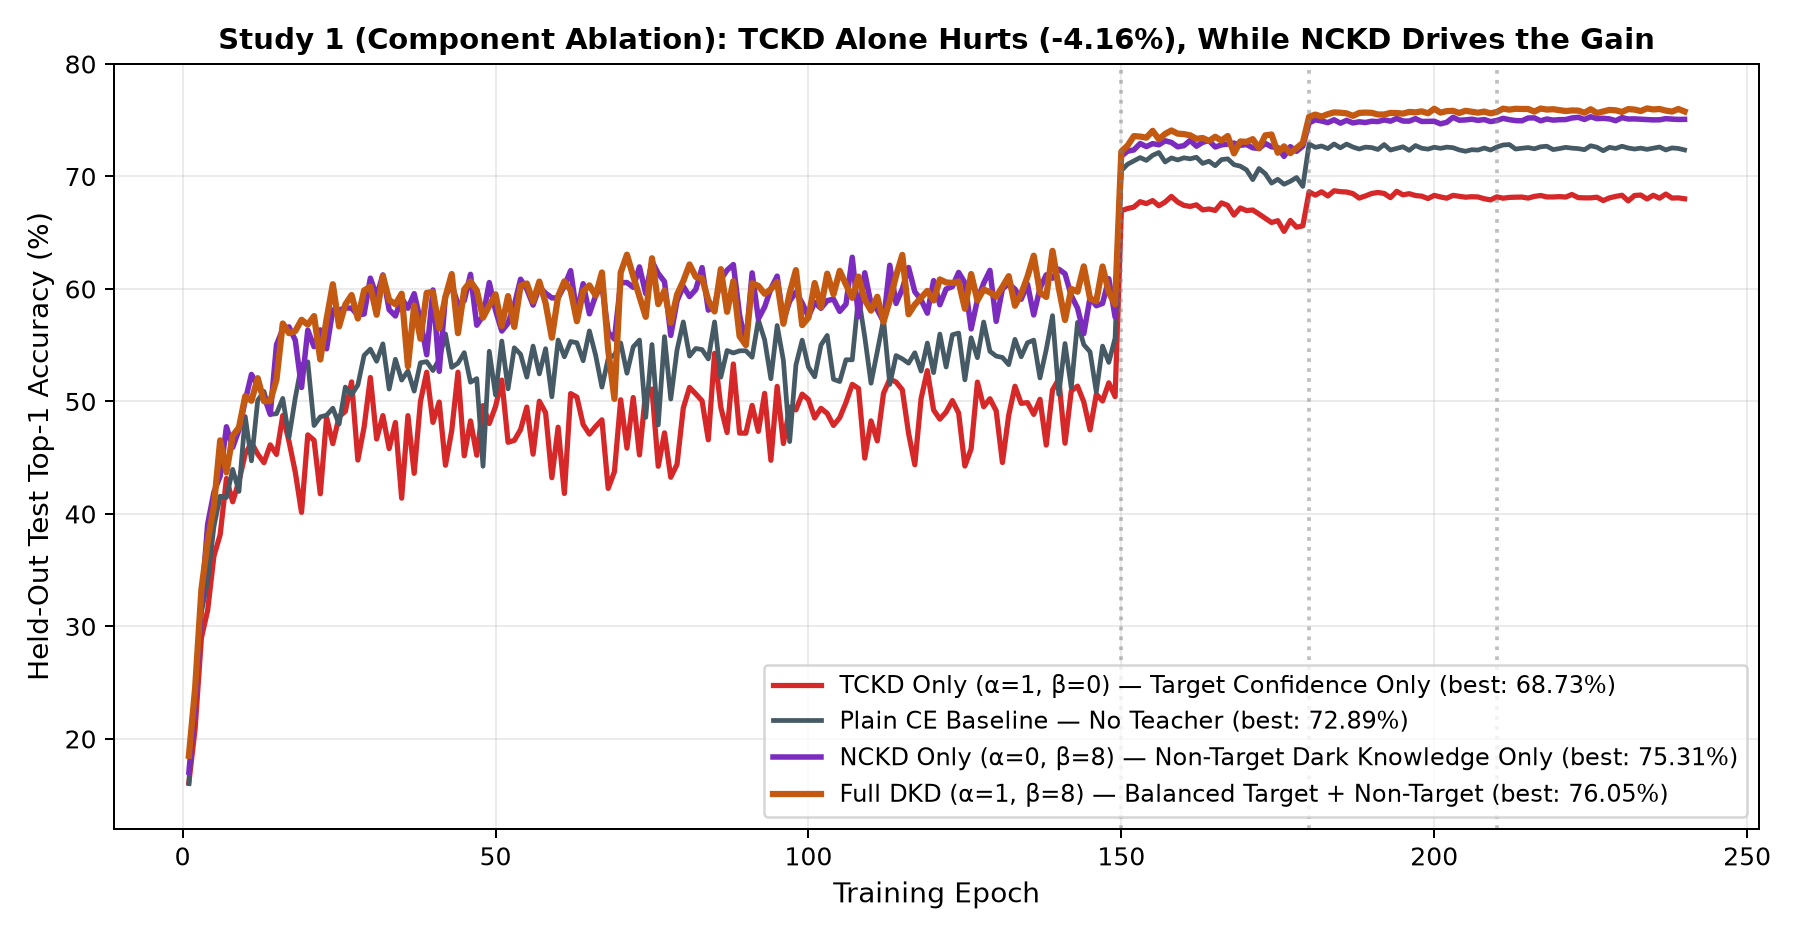
\includegraphics[width=0.91\textwidth]{component_ablation_curves.png}
\caption{Study 1 trajectories: \texttt{TCKD} alone falls below Plain CE, whereas \texttt{NCKD} accounts for the bulk of DKD's accuracy gain.}
\label{fig:ablation_curves}
\end{figure}

\begin{figure}[!htbp]
\centering
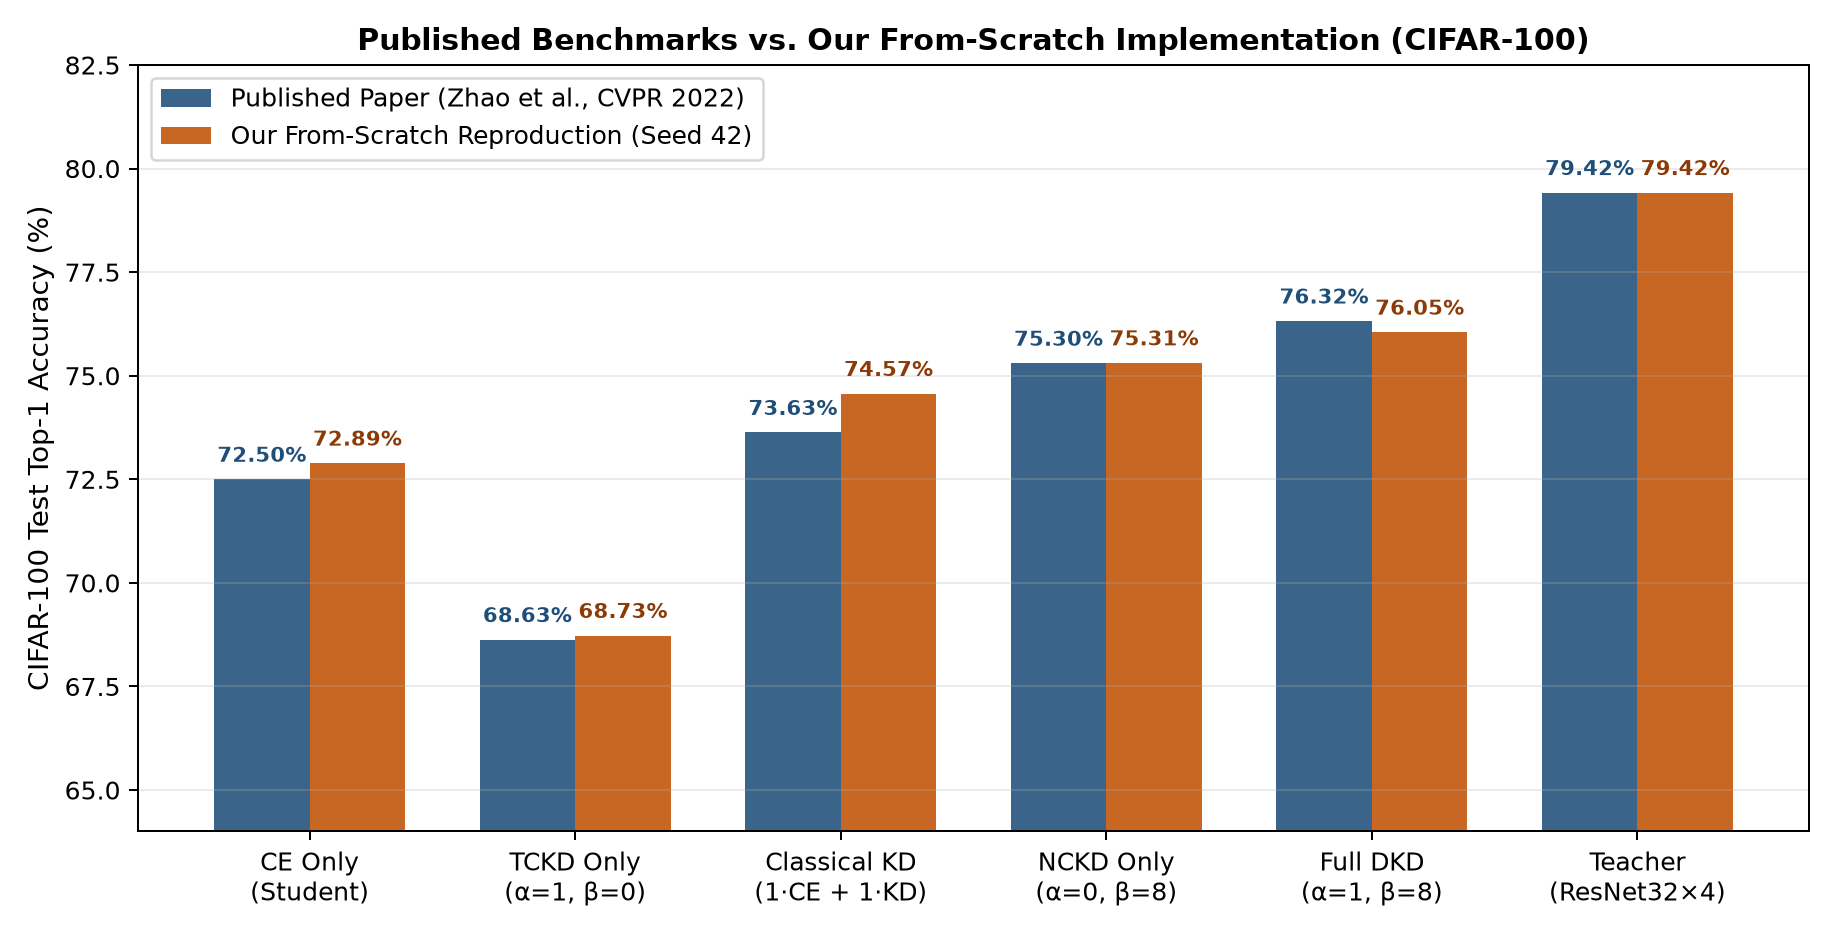
\includegraphics[width=0.91\textwidth]{paper_vs_ours_bars.png}
\caption{Published CVPR 2022 numbers vs.\ our \texttt{SEED=42} from-scratch suite across all six baseline and ablation settings.}
\label{fig:bars_all}
\end{figure}

\subsection{Study 2: Head-to-Head Temperature Sweep and High-Temperature Limit}

\begin{itemize}
    \item \textbf{Research Question:} How sensitive are Classical KD and DKD to the softmax temperature \(T\), particularly at unsoftened \(T=1.0\) and extreme \(T=100.0\)?
    \item \textbf{Setup:} Under the same \texttt{SEED=42} protocol, we trained Classical KD at \(T \in \{1.0, 4.0, 10.0\}\) (\texttt{kd\_T1}, \texttt{kd\_T4}, \texttt{kd\_T10}) and DKD (\(\alpha=1, \beta=8\)) at \(T \in \{1.0, 4.0, 10.0, 100.0\}\) (\texttt{dkd\_T1}, \texttt{dkd\_T4}, \texttt{dkd\_T10}, \texttt{dkd\_T100}).
    \item \textbf{Results (Table~\ref{tab:temp}, Figure~\ref{fig:temp_sweep}):}
    \begin{enumerate}
        \item \textbf{Collapse of Classical KD at \(T=1.0\):} Without temperature softening, \(p_t^T \approx 0.999\) makes \((1 - p_t^T) \approx 0.001\). \texttt{kd\_T1} drops to \(72.95\%\) (last-20 mean \(72.41\%\)), essentially tied with plain \texttt{ce} (\(72.89\%\)) while overfitting training data (\(97.04\%\) train accuracy). At the same \(T=1.0\), \texttt{dkd\_T1} reaches \(75.61\%\), beating \texttt{kd\_T1} by \(+2.66\%\) and beating softened \texttt{kd\_T4} (\(74.57\%\)) by \(+1.04\%\).
        \item \textbf{Stability Across \(T=4\text{--}10\) and Bend at \(T=100\):} DKD stays between \(76.05\%\) (\(T=4.0\)) and \(76.28\%\) (\(T=10.0\)). Raising temperature to \(T=100.0\) (\texttt{dkd\_T100}) remains numerically stable (zero NaNs due to \(T^2 = 10{,}000\) scaling) and reaches \(75.84\%\), dipping by \(0.44\%\) below \(T=10.0\).
    \end{enumerate}
\end{itemize}

\begin{table}[!htbp]
\centering
\small
\caption{Study 2: Classical KD vs.\ DKD Across Softmax Temperatures \(T \in [1, 100]\) (\texttt{SEED=42}).}
\label{tab:temp}
\resizebox{\textwidth}{!}{%
\begin{tabular}{@{}lcccccc@{}}
\toprule
\textbf{Temperature \(T\)} & \textbf{KD Best Top-1} & \textbf{KD Last-20} & \textbf{DKD Best Top-1} & \textbf{DKD Last-20} & \textbf{DKD Gain Over KD} \\
\midrule
\(T = 1.0\) (Sharp / Unsoftened) & \(72.95\%\) & \(72.41\%\) & \textbf{75.61\%} & \(75.39\%\) & \textbf{+2.66\%} \\
\(T = 4.0\) (Paper Standard) & \(74.57\%\) & \(74.30\%\) & \textbf{76.05\%} & \(75.87\%\) & \textbf{+1.48\%} \\
\(T = 10.0\) (High Softening) & \(74.45\%\) & \(74.22\%\) & \textbf{76.28\%} & \(76.04\%\) & \textbf{+1.83\%} \\
\(T = 100.0\) (Asymptotic Limit) & -- & -- & \textbf{75.84\%} & \(75.70\%\) & -- \\
\bottomrule
\end{tabular}}
\end{table}

\begin{figure}[!htbp]
\centering
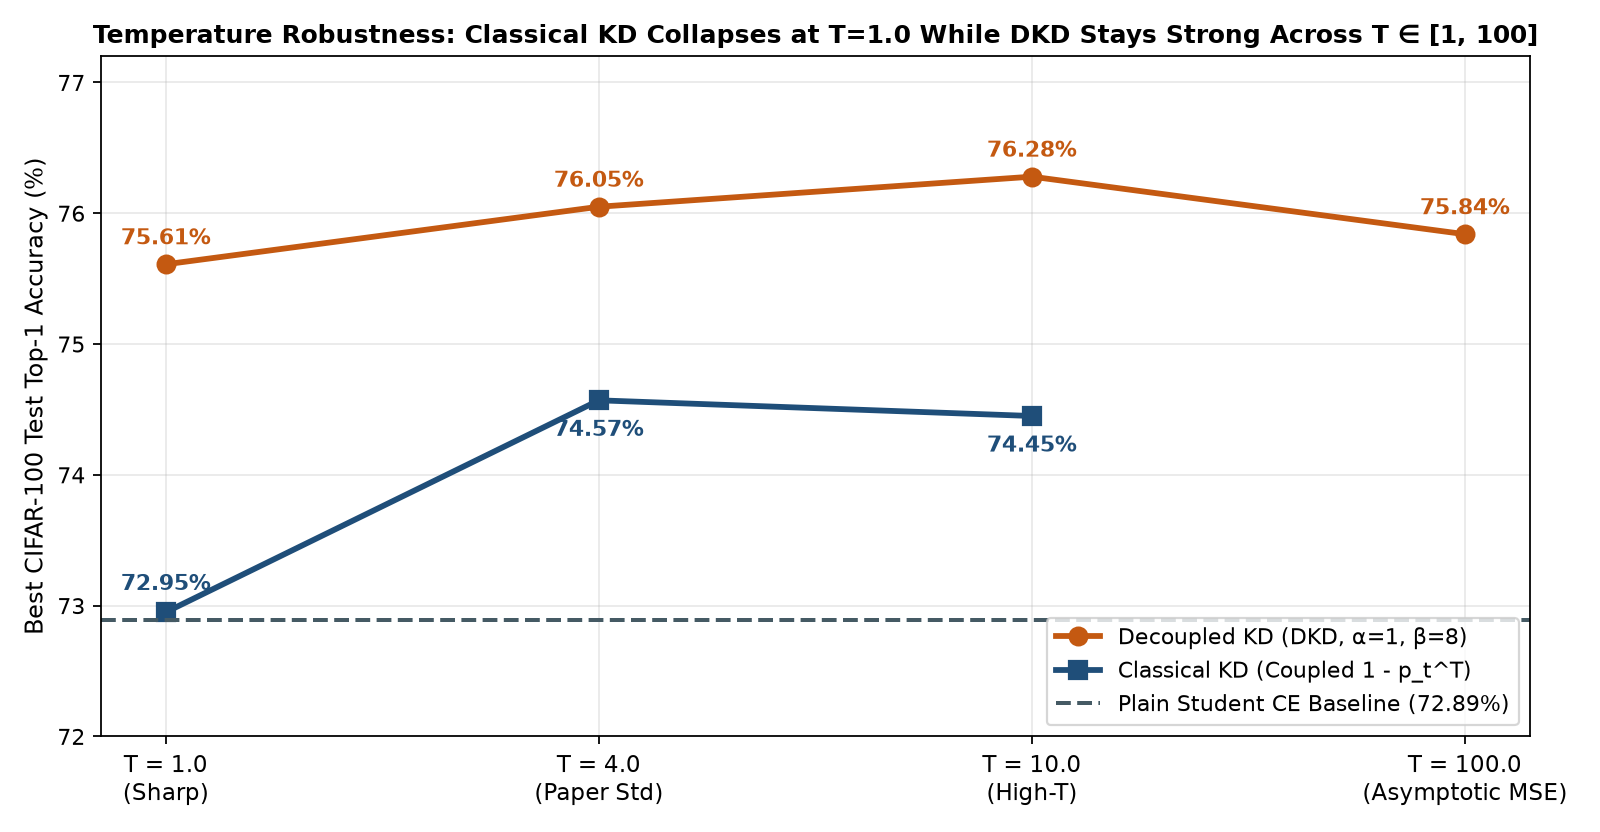
\includegraphics[width=0.92\textwidth]{kd_vs_dkd_temperature_sweep.png}
\caption{Study 2: Classical KD collapses to the plain CE baseline at \(T=1.0\), while DKD remains above \(75.6\%\) across two orders of magnitude in \(T\).}
\label{fig:temp_sweep}
\end{figure}

\subsection{Study 3: Training Step Cost and Inference Compression}

\begin{itemize}
    \item \textbf{Research Question:} How much training time does DKD add over Classical KD, and what size and latency reductions are achieved at test time?
    \item \textbf{Results (Figure~\ref{fig:compute}):} Over 240 epochs (\(187{,}680\) batches of 64) on an NVIDIA L4 GPU, plain \texttt{ce} averages \(9.54\text{ ms/batch}\) (\(29.8\text{ min}\) total). Adding the frozen teacher forward pass brings \texttt{kd\_T4} to \(18.30\text{ ms/batch}\) (\(57.2\text{ min}\)) and \texttt{dkd\_T4} to \(18.87\text{ ms/batch}\) (\(59.0\text{ min}\)), a difference of \(+0.57\text{ ms/batch}\) (\(\approx 3\%\)) for logit masking. At deployment, discarding the teacher shrinks model size by \(6.03\times\) (\(28.36\text{ MB} \to 4.71\text{ MB}\)) and speeds up single-image CPU forward passes by \(2.6\times\) (\(9.92\text{ ms} \to 3.80\text{ ms}\)).
\end{itemize}

\begin{figure}[!htbp]
\centering
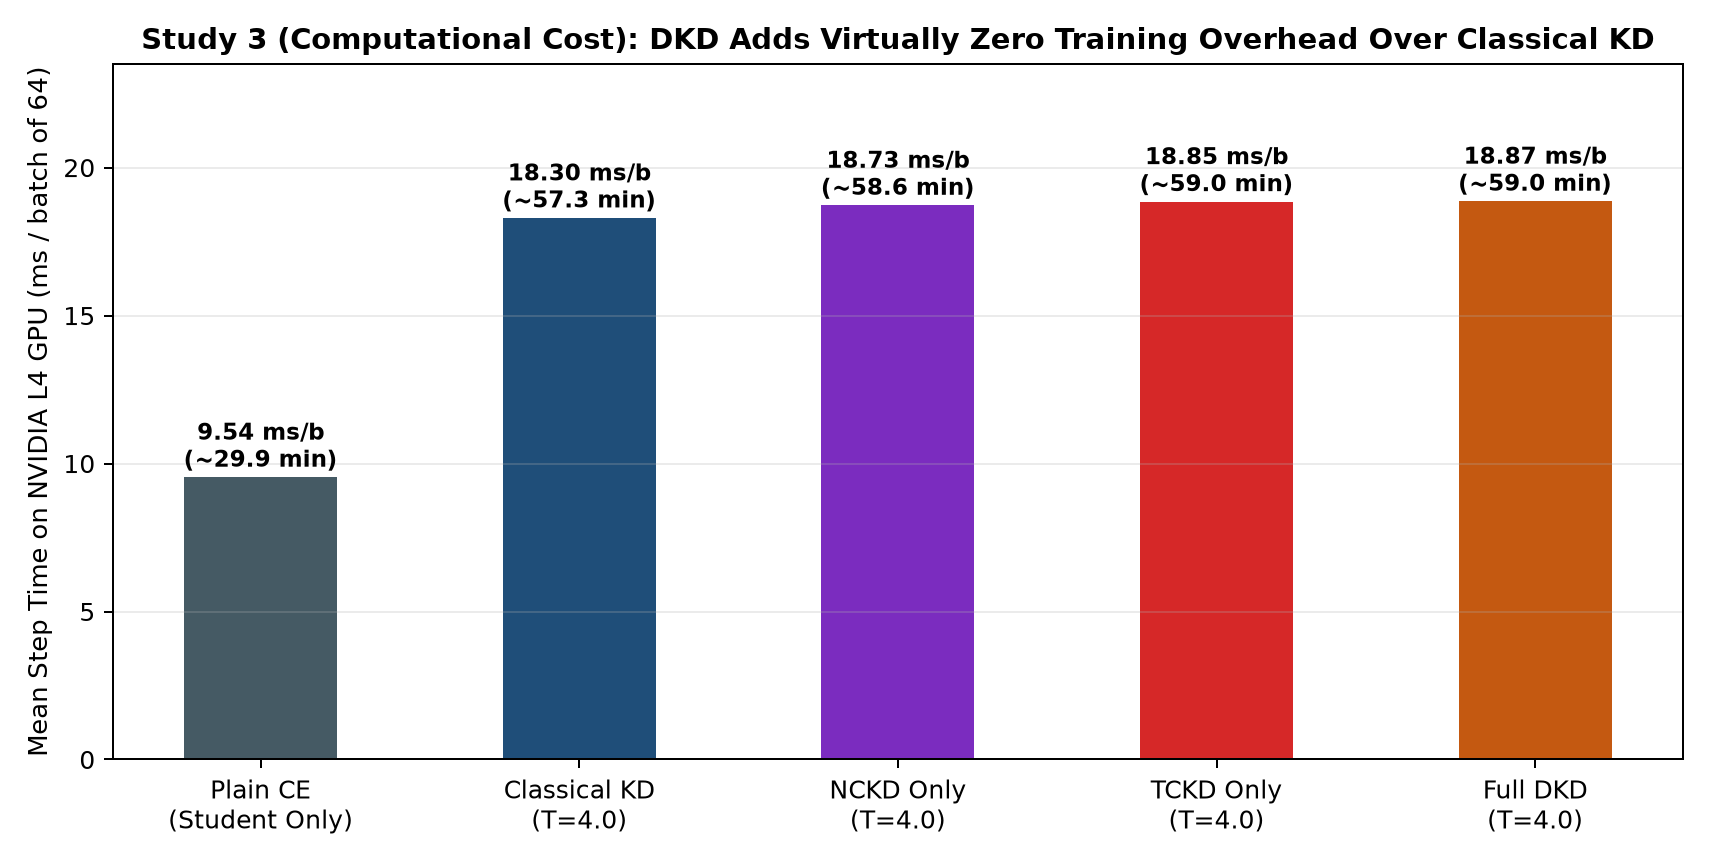
\includegraphics[width=0.86\textwidth]{computational_efficiency.png}
\caption{Study 3: Mean per-batch training time on NVIDIA L4 GPU across all five loss modes.}
\label{fig:compute}
\end{figure}

% =====================================================================
\section{Analysis and Discussion}
\label{sec:discussion}

\begin{enumerate}
    \item \textbf{Teacher-Gap Closure vs.\ Raw Accuracy:} Raw percentage gains look modest only if compared against \(100\%\) rather than the teacher's \(79.42\%\) ceiling. Above our \(72.89\%\) label-only student, the total teacher--student gap is \(6.53\) points. Classical KD closes \(25.7\%\) of that gap (\(+1.68\) points), whereas DKD closes \(48.4\%\) on Seed 1 and \(54.5\%\) on Seed 2 (\(51.5\%\) mean), transferring roughly twice as much of the teacher's advantage into the same \(4.71\text{ MB}\) network.
    \item \textbf{Signal vs.\ Single-Seed Variance:} On a \(10{,}000\)-image test set (\(1\% = 100\) images), separate SGD runs with random crops and flips vary by \(\sigma \approx \pm 0.25\%\). Our two \(T=4.0\) DKD runs (\(76.05\%\) with \texttt{kaiming\_uniform\_} and \(76.45\%\) with \texttt{kaiming\_normal\_}, mean \(76.25\%\)) bracket the paper's 5-trial mean (\(76.32\%\)) within \(1\sigma\). By contrast, DKD's \(+1.48\%\) to \(+2.66\%\) lead over Classical KD across \(T \in \{1, 4, 10\}\) exceeds \(5\sigma\). Our \texttt{kd\_T4} baseline (\(74.57\%\)) also ran slightly above Paper Table~1 (\(73.63\%\)), making our measured DKD gain conservative.
    \item \textbf{Regularization Against Label Memorization:} Figure~\ref{fig:gen_gap} compares training and test accuracy at Epoch 240. Plain \texttt{ce} (\(95.32\%\) train vs.\ \(72.36\%\) test) and \texttt{kd\_T1} (\(97.04\%\) train vs.\ \(72.36\%\) test) memorize one-hot training labels, leaving \(23\%\text{--}25\%\) train--test gaps. Enforcing \(\beta = 8.0\) on \(\mathrm{NCKD}\) requires each 256-D image embedding to satisfy 99 non-target similarity targets simultaneously, holding training accuracy near \(88\%\text{--}90\%\) and narrowing the train--test gap to \(14.2\%\).
    \item \textbf{Asymptotic Behavior at \(T=10\) and \(T=100\):} For \(|z_i|/T \ll 1\), first-order Taylor expansion \(\exp(z_i/T) \approx 1 + z_i/T\) implies that \(T^2\,\mathrm{NCKD}\) approaches \(L_2\) mean-squared error (MSE) across the 99 mean-centered non-target logits, while binary \(\mathrm{TCKD}\) approaches \(p_t \approx 1/C\) \cite{hinton2015}. Because \texttt{ResNet8$\times$4} shares identical stage widths \([64, 128, 256]\) with \texttt{ResNet32$\times$4}, direct non-target logit matching works well at \(T=10\) (\(76.28\%\)). At \(T=100\), however, softmax no longer attenuates large negative logits on unrelated classes (for example, matching whether \texttt{skyscraper} is \(-8.1\) vs.\ \(-4.9\) on a \texttt{crocodile} image), which dilutes gradient focus on plausible cousin classes and lowers accuracy to \(75.84\%\). \(T=4.0\) balances both regimes: soft enough to expose related classes while still zeroing out negative-logit noise.
\end{enumerate}

\begin{figure}[!htbp]
\centering
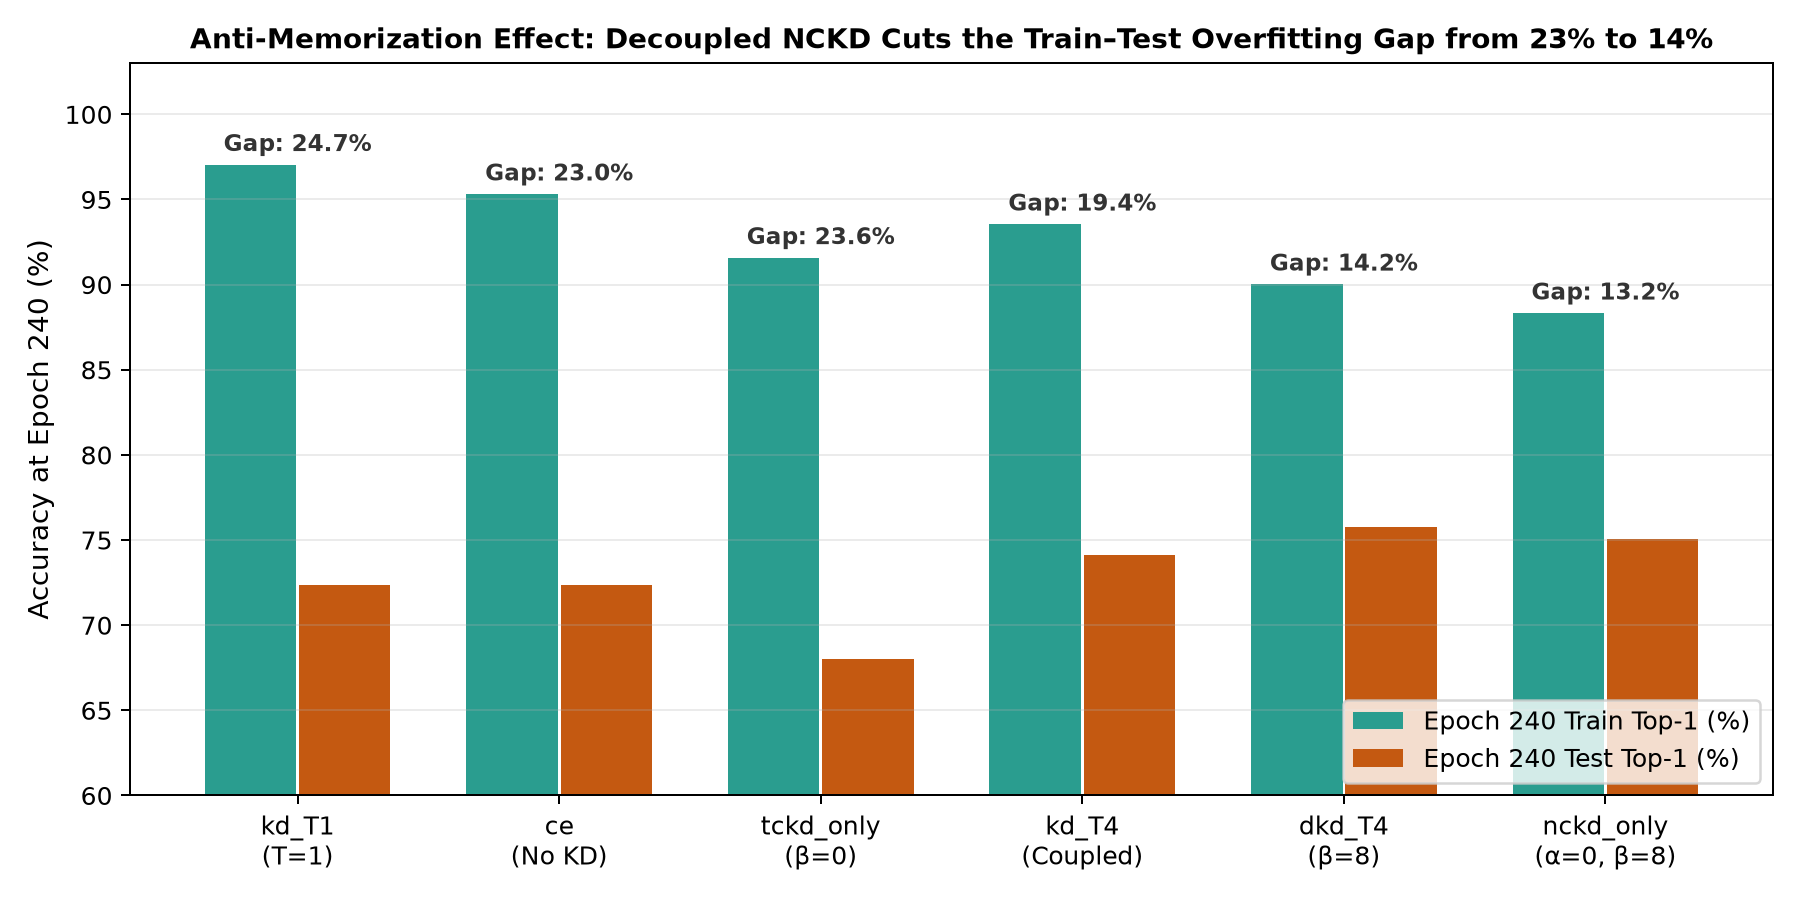
\includegraphics[width=0.90\textwidth]{generalization_gap_bars.png}
\caption{Epoch 240 training vs.\ test accuracy: decoupled \texttt{NCKD} (\(\beta=8\)) reduces one-hot label memorization.}
\label{fig:gen_gap}
\end{figure}

\clearpage
% =====================================================================
\section{Model Deployment}
\label{sec:deploy}

\subsection{Inference Pipeline and Input/Output Contract}

All eleven trained \texttt{ResNet8$\times$4} checkpoints and the frozen \texttt{ResNet32$\times$4} teacher are served in a standalone Streamlit application (\texttt{app.py}), hosted publicly on Streamlit Community Cloud (\url{\LiveAppURL}) and runnable offline on local machines:
\[
\text{Input} \rightarrow 32{\times}32\text{ RGB \& Norm} \rightarrow \text{Frozen \texttt{ResNet8$\times$4}} \rightarrow \text{Top-5 \& \texttt{NCKD}} \rightarrow \text{UI}.
\]
\begin{itemize}
    \item \textbf{Inputs:} (1) Any of the \(10{,}000\) held-out CIFAR-100 test images (via class filter, sample index, random draw, or 1-click presets), or (2) user-uploaded \texttt{.png}, \texttt{.jpg}, \texttt{.jpeg}, or \texttt{.webp} files (alongside \(10{,}000\) lossless test PNGs exported via \texttt{scripts/export\_test\_images.py} for live upload testing).
    \item \textbf{Preprocessing:} Converts images to RGB, bilinearly resizes non-\(32\times 32\) uploads to \(32 \times 32\), normalizes by CIFAR-100 \(\mu, \sigma\), and builds a contiguous \texttt{float32} tensor of shape \((1, 3, 32, 32)\).
    \item \textbf{Outputs:} Top-1 predicted label, ground-truth check badge, confidence (\%), 20-pass mean latency (\(\text{ms}\)), Plotly top-5 probability charts, a live \((1 - p_t^T)\) vs.\ \(\beta=8.0\) non-target dark-knowledge microscope (\texttt{NCKD}), and an interactive multi-run leaderboard.
\end{itemize}

\subsection{Setup, Startup Instructions, and Dependencies}

From a fresh clone of \url{\RepoURL} with Python \(3.11+\) (dependencies pinned in \texttt{requirements.txt}: PyTorch 2.15.0, Streamlit 1.67.0, Plotly 7.1.0, NumPy 2.5.4, Pillow 13.0.0):
\begin{verbatim}
python3 scripts/setup_project.py  # Builds .venv & verifies CIFAR-100
.venv/bin/streamlit run app.py    # Launches UI at http://localhost:8501
\end{verbatim}
On Streamlit Community Cloud, \texttt{app.py} caches models via \texttt{@st.cache\_resource} and automatically downloads CIFAR-100 and the teacher checkpoint on initial container boot.

\subsection{Example Inference Walkthrough and Application Screenshots}

On held-out CIFAR-100 Test Image \texttt{\#428} (ground truth: \texttt{crocodile}, superclass: \texttt{reptiles}), the deployed \(4.71\text{ MB}\) \texttt{dkd\_T4} student predicts \textbf{\texttt{crocodile} (\(82.8\%\) confidence)} in \textbf{\(3.80\text{ ms}\)} on CPU, compared to \(9.92\text{ ms}\) for the \(28.36\text{ MB}\) teacher (\(99.6\%\) confidence). Selecting the plain \texttt{ce} student checkpoint in the sidebar on the same image flips the prediction to \textbf{\texttt{bear} (\(70.8\%\))}, illustrating DKD's decision improvement directly in the interface (Figures~\ref{fig:ui_overview}--\ref{fig:ui_leaderboard}).

\begin{figure}[!htbp]
\centering
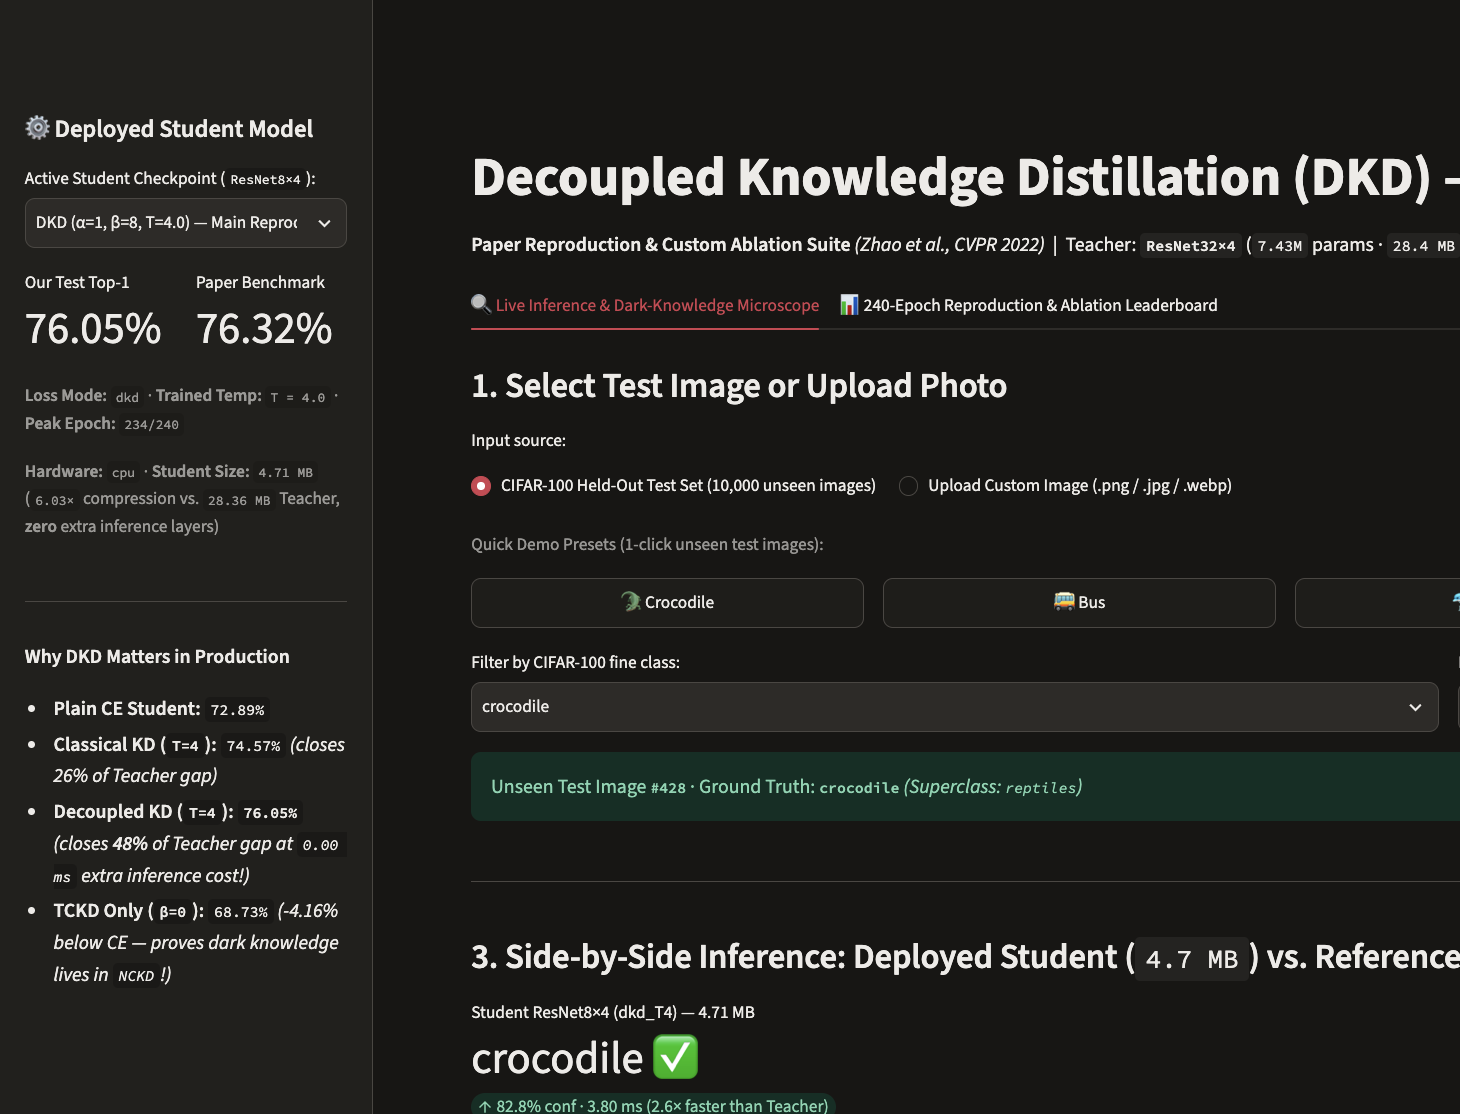
\includegraphics[width=0.95\textwidth]{app_live_overview.png}
\caption{Deployed Streamlit app (\texttt{app.py}, Tab 1): checkpoint selector, input controls, \(32\times 32\) preprocessing view, and side-by-side inference on Test Image \texttt{\#428} (\texttt{crocodile}).}
\label{fig:ui_overview}
\end{figure}

\begin{figure}[!htbp]
\centering
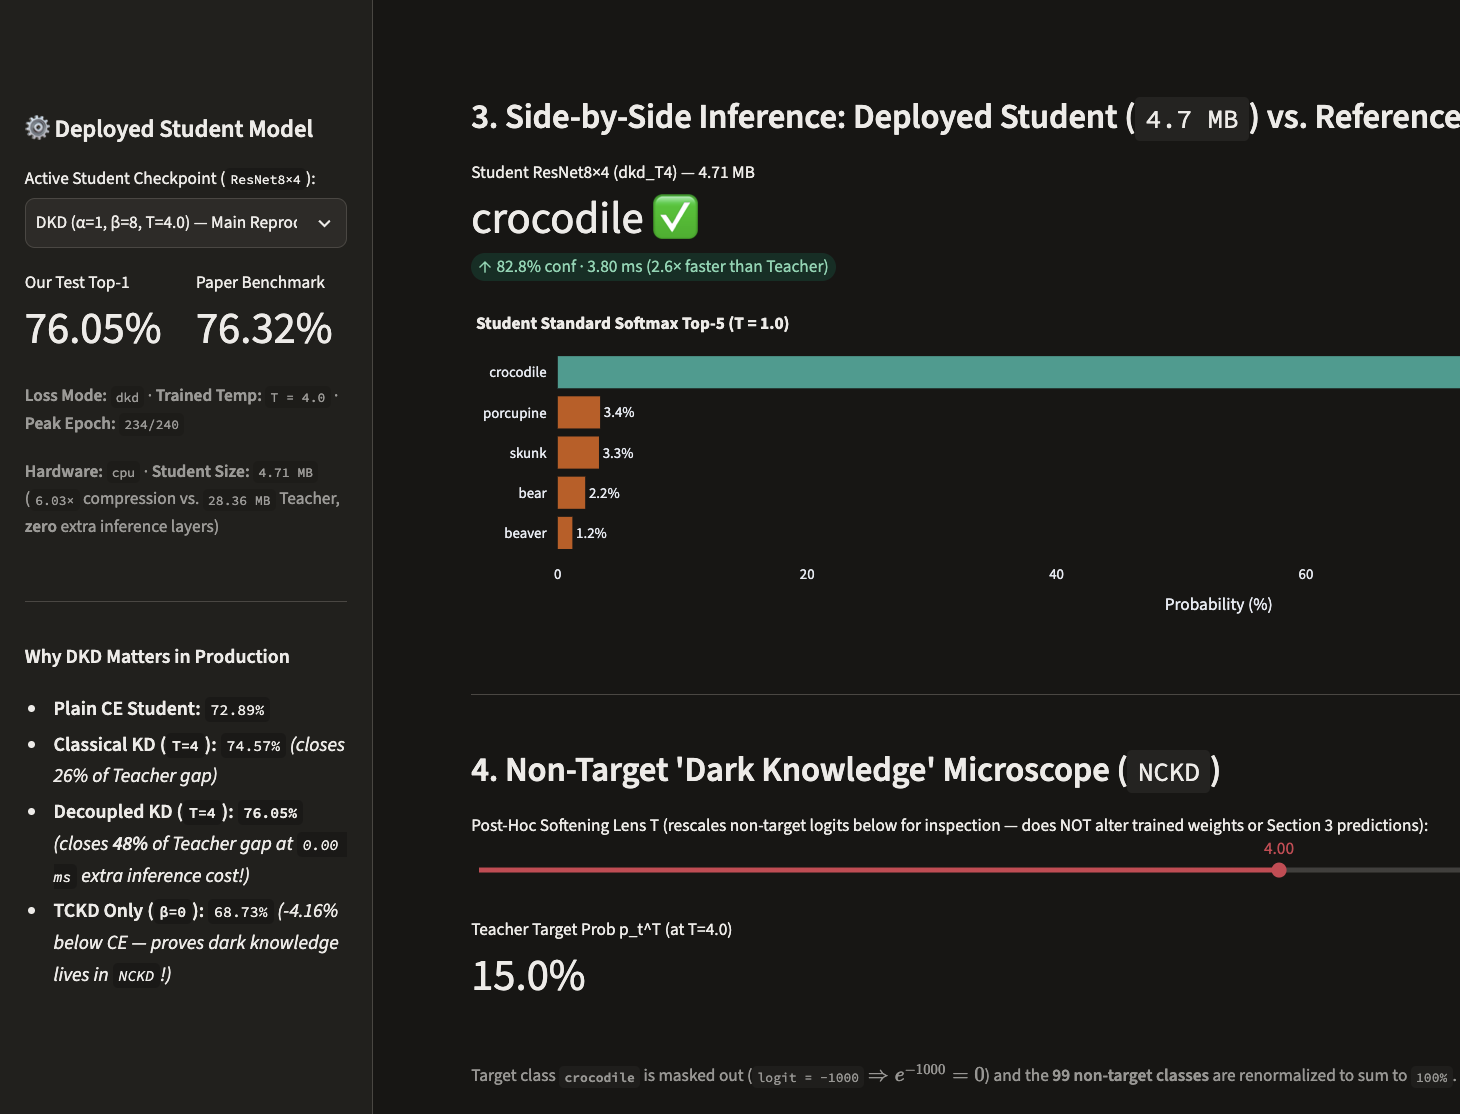
\includegraphics[width=0.95\textwidth]{app_nckd_microscope.png}
\caption{Tab 1 Prediction \& Section 4 Dark-Knowledge Microscope comparing Classical KD's coupled weight \((1 - p_t^T) = 0.850\times\) against DKD's \(\beta = 8.000\times\) (\(9.4\times\) stronger non-target weight).}
\label{fig:ui_microscope}
\end{figure}

\begin{figure}[!htbp]
\centering
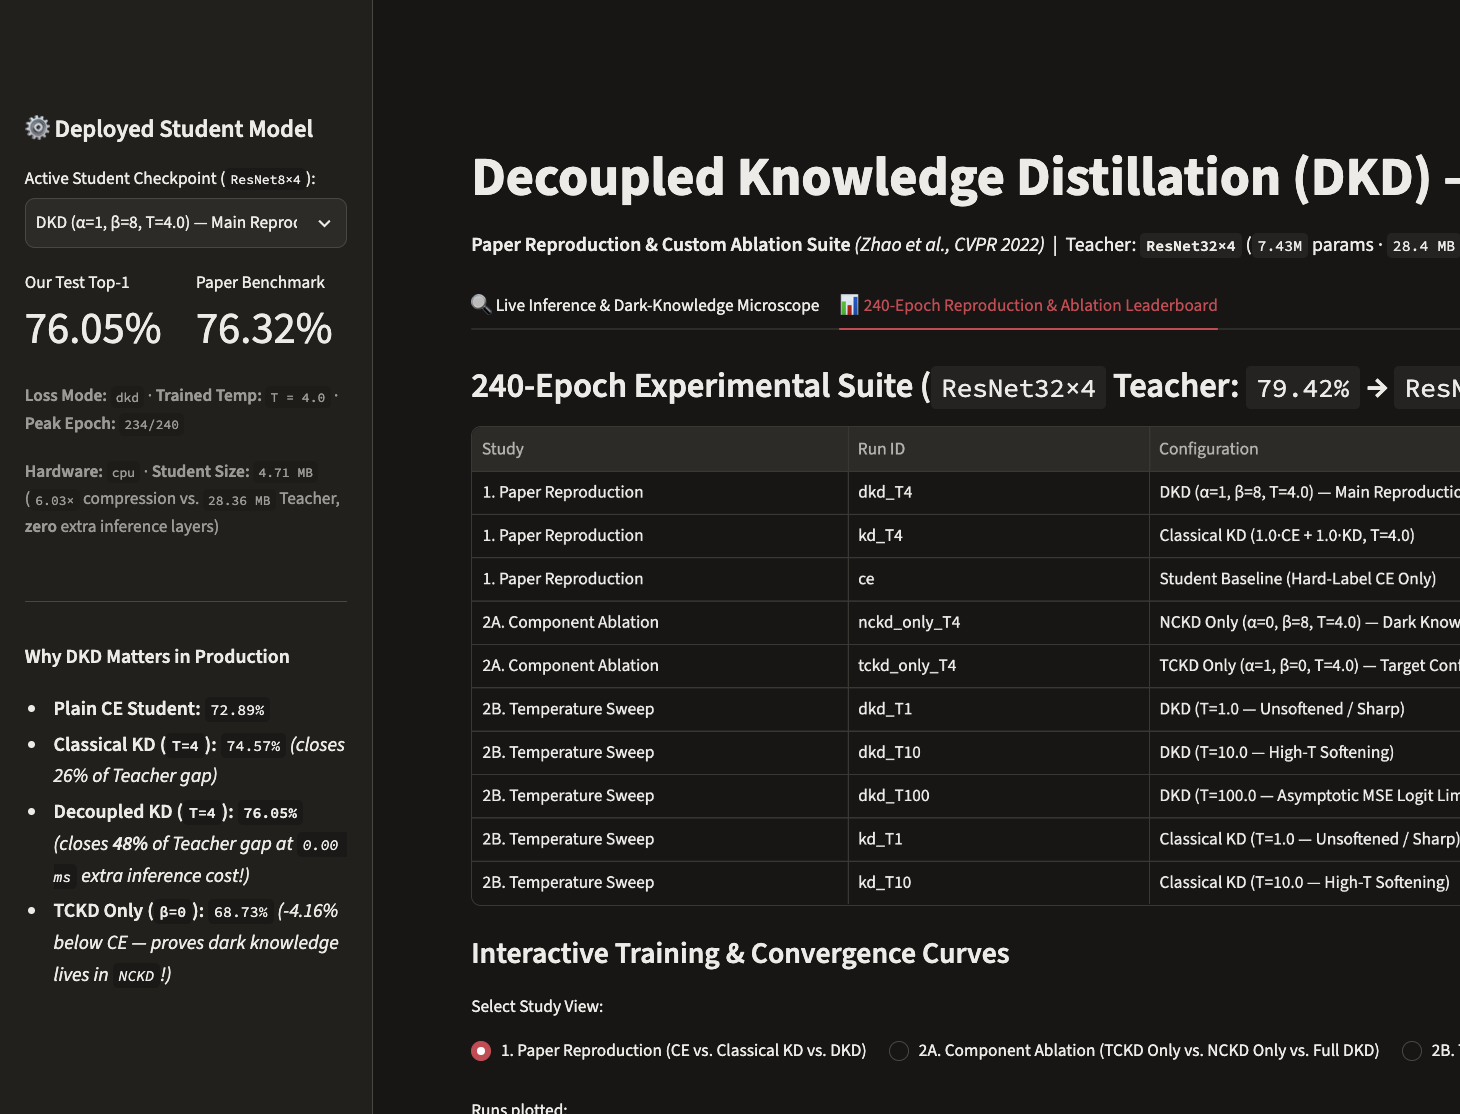
\includegraphics[width=0.95\textwidth]{app_leaderboard.png}
\caption{Tab 2 Study Explorer: 240-epoch leaderboard with paper benchmarks, teacher-gap closure, step times, and filterable accuracy curves.}
\label{fig:ui_leaderboard}
\end{figure}

% =====================================================================
\section{Limitations}
\label{sec:limits}

\begin{enumerate}
    \item \textbf{No Spatial Supervision for Detection or Segmentation:} Because DKD acts only on pooled \((B, C)\) logits, it transfers no \((H \times W)\) spatial localization cues. On MS-COCO detection, Zhao et al.\ combined DKD with feature review rather than using logit distillation alone \cite{zhao2022}.
    \item \textbf{\(32 \times 32\) Input Bottleneck on High-Resolution Photos:} Because \texttt{AvgPool2d(8)} expects an \(8 \times 8\) feature map before \texttt{fc}, uploaded photos must be resized to \(32 \times 32\), losing fine detail and limiting outputs to CIFAR-100's 100 classes.
    \item \textbf{Homogeneous Backbone Scope:} While primary \(T=4.0\) DKD was verified across two independent seeds (\texttt{dkd\_T4} and \texttt{dkd\_T4\_seed2}), the ablation and temperature sweeps used a single controlled seed (\texttt{SEED=42}) on one same-family pair (\(\texttt{ResNet32$\times$4} \to \texttt{ResNet8$\times$4}\)). Cross-architecture pairs (such as \(\texttt{ResNet50} \to \texttt{MobileNetV2}\)) may degrade earlier at \(T \ge 10\) when linear head geometries differ.
    \item \textbf{Training-Time Teacher Pass \& \(\beta\) Selection:} Although test-time inference uses only the student, training still runs a teacher forward pass every batch (\(\approx 1.9\times\) slower than plain CE), and optimal \(\beta\) varies with teacher confidence across datasets (\(\beta = 8\) on CIFAR-100 vs.\ \(\beta = 2\) on ImageNet \cite{zhao2022}).
\end{enumerate}

% =====================================================================
\section{Conclusion}
\label{sec:conclusion}

We implemented, ablated, and deployed \emph{Decoupled Knowledge Distillation} (Zhao et al., CVPR 2022) from scratch on CIFAR-100. Separating classical KD into target-class confidence (\(\mathrm{TCKD}\)) and 99-class conditional non-target similarity (\(\mathrm{NCKD}\)) confirmed both algebraically and empirically why the classical \((1 - p_t^T)\) factor suppresses dark knowledge. Across audited 240-epoch checkpoints, our distilled \texttt{ResNet8$\times$4} student reached \(76.05\%\) and \(76.45\%\) top-1 accuracy (\(76.25\%\) mean vs.\ \(76.32\%\) published), closing roughly half of the teacher--student gap while shrinking checkpoint size by \(6.03\times\) (\(4.71\text{ MB}\)) and accelerating CPU inference by \(2.6\times\). Our additional experiments showed that \(\mathrm{TCKD}\) alone drops accuracy below plain cross-entropy (\(68.73\%\)), \(\mathrm{NCKD}\) alone exceeds classical KD (\(75.31\%\)), and decoupling eliminates classical KD's collapse at \(T=1.0\) (\(75.61\%\) vs.\ \(72.95\%\)).

% =====================================================================
\section{References}
\label{sec:refs}

\begingroup
\renewcommand{\section}[2]{}%
\begin{thebibliography}{99}

\bibitem{zhao2022}
B.~Zhao, Q.~Cui, R.~Song, Y.~Qiu, and J.~Liang, ``Decoupled knowledge distillation,'' in \emph{Proc.\ IEEE/CVF Conf.\ Comput.\ Vis.\ Pattern Recognit.\ (CVPR)}, New Orleans, LA, USA, 2022, pp.\ 11953--11962.

\bibitem{hinton2015}
G.~Hinton, O.~Vinyals, and J.~Dean, ``Distilling the knowledge in a neural network,'' \emph{arXiv preprint arXiv:1503.02531}, 2015.

\bibitem{romero2015}
A.~Romero, N.~Ballas, S.~E.~Kahou, A.~Chassang, C.~Gatta, and Y.~Bengio, ``FitNets: Hints for thin deep nets,'' in \emph{Proc.\ Int.\ Conf.\ Learn.\ Represent.\ (ICLR)}, 2015.

\bibitem{zagoruyko2017}
S.~Zagoruyko and N.~Komodakis, ``Paying more attention to attention: Improving the performance of convolutional neural networks via attention transfer,'' in \emph{Proc.\ Int.\ Conf.\ Learn.\ Represent.\ (ICLR)}, 2017.

\bibitem{park2019}
W.~Park, D.~Kim, Y.~Lu, and M.~Cho, ``Relational knowledge distillation,'' in \emph{Proc.\ IEEE/CVF Conf.\ Comput.\ Vis.\ Pattern Recognit.\ (CVPR)}, 2019, pp.\ 3967--3976.

\bibitem{tian2020}
Y.~Tian, D.~Krishnan, and P.~Isola, ``Contrastive representation distillation,'' in \emph{Proc.\ Int.\ Conf.\ Learn.\ Represent.\ (ICLR)}, 2020.

\bibitem{heo2019}
B.~Heo, J.~Kim, S.~Yun, H.~Park, N.~Kwak, and J.~Y.~Choi, ``A comprehensive overhaul of feature distillation,'' in \emph{Proc.\ IEEE/CVF Int.\ Conf.\ Comput.\ Vis.\ (ICCV)}, 2019, pp.\ 1921--1930.

\bibitem{chen2021}
P.~Chen, S.~Liu, H.~Zhao, and J.~Jia, ``Distilling knowledge via knowledge review,'' in \emph{Proc.\ IEEE/CVF Conf.\ Comput.\ Vis.\ Pattern Recognit.\ (CVPR)}, 2021, pp.\ 5008--5017.

\bibitem{zhang2018}
Y.~Zhang, T.~Xiang, T.~M.~Hospedales, and H.~Lu, ``Deep mutual learning,'' in \emph{Proc.\ IEEE/CVF Conf.\ Comput.\ Vis.\ Pattern Recognit.\ (CVPR)}, 2018, pp.\ 4320--4328.

\bibitem{mirzadeh2020}
S.~I.~Mirzadeh, M.~Farajtabar, A.~Li, N.~Levine, A.~Matsukawa, and H.~Ghasemzadeh, ``Improved knowledge distillation via teacher assistant,'' in \emph{Proc.\ AAAI Conf.\ Artif.\ Intell.}, 2020, pp.\ 5191--5198.

\bibitem{cho2019}
J.~H.~Cho and B.~Hariharan, ``On the efficacy of knowledge distillation,'' in \emph{Proc.\ IEEE/CVF Int.\ Conf.\ Comput.\ Vis.\ (ICCV)}, 2019, pp.\ 4794--4802.

\bibitem{krizhevsky2009}
A.~Krizhevsky, ``Learning multiple layers of features from tiny images,'' University of Toronto, Tech.\ Rep., 2009.

\bibitem{bucilua2006}
C.~Bucilu\u{a}, R.~Caruana, and A.~Niculescu-Mizil, ``Model compression,'' in \emph{Proc.\ 12th ACM SIGKDD Int.\ Conf.\ Knowl.\ Discovery Data Mining (KDD)}, 2006, pp.\ 535--541.

\bibitem{he2016}
K.~He, X.~Zhang, S.~Ren, and J.~Sun, ``Deep residual learning for image recognition,'' in \emph{Proc.\ IEEE Conf.\ Comput.\ Vis.\ Pattern Recognit.\ (CVPR)}, 2016, pp.\ 770--778.

\end{thebibliography}
\endgroup

\appendix
\section{Summary of Revisions from Deliverable 2 (Mid-Evaluation Report)}
\label{app:revisions}

Per Section 2.3 of the Deliverable 3 guidelines, the following additions and refinements were made relative to Deliverable 2:
\begin{itemize}
    \item \textbf{Carried Over \& Refined (Sections~\ref{sec:lit} and \ref{sec:eda}):} Retained the Deliverable 2 Literature Review and all nine CIFAR-100 EDA figures and exact statistics, updating future tense to completed experiments and connecting intra-superclass visual similarity to \(\mathrm{NCKD}\).
    \item \textbf{Added Methodology \& Implementation Details (Sections~\ref{sec:method} and \ref{sec:impl}):} Added the algebraic derivation of Equation~\eqref{eq:exact_kd}, the \(-1000.0\) logit-masking stability analysis, stage-by-stage ResNet tensor/shortcut diagrams, conv initialization details, and the 4-part Code \& Result Attribution table.
    \item \textbf{Added Reproduction, Custom Studies, and Deployment (Sections~\ref{sec:repro}--\ref{sec:limits}):} Integrated all eleven 240-epoch checkpoints in \texttt{outputs\_final/} (two \texttt{dkd\_T4} seeds plus \texttt{ce}, \texttt{kd\_T1/T4/T10}, \texttt{tckd\_only\_T4}, \texttt{nckd\_only\_T4}, and \texttt{dkd\_T1/T10/T100}), train--test gap and high-\(T\) limit analysis, and live Streamlit deployment documentation.
\end{itemize}

\end{document}
